\chapter{Results and Evaluation} \label{chap:result}
%{\color{red}Give some introduction, the structure of this chapter.}
\textbf{Parameter setup}
First of all, we need to specify the parameters we used throughout the whole evaluation part. 
The default parameters are used for the RGBD-Fusion method, which has 8 in total. 
It should be mentioned that, since both proposed methods don't have a smoothness term for the depth enhancement, $\lambda_z^2$ in RGBD-Fusion and $\lambda_l$ in our RGBD-Fusion Like method are set to 0 for the sake of fairness of comparison.
$\lambda_z^2$ and $\lambda_l$ are set to the values in table~\ref{tab:parameter_setup} only during the quantitative evalution because we want to illustrate the importance of this depth smoothness term for the RGBD-Fusion method.
\begin{table}[!ht]
\caption{Parameters of all the methods used throughout all the experiments.}
\label{tab:parameter_setup}
\centering
\begin{tabular}{|m{4cm} |m{1.5cm} |m{7cm}|}
\hline
\multicolumn{1}{|c|}{Method}                               & \multicolumn{1}{c|}{Total number} & \multicolumn{1}{c|}{Parameters}                                                                                                                                          \\ \hline
RGBD-Fusion~\cite{or2015rgbd} & \multicolumn{1}{c|}{8}            &{$\lambda_\rho = 0.1, \lambda_\beta^1 = 0.1, \lambda_\beta^2 = 0.1, \tau = 0.05, \sigma_c = \sqrt{0.05}, \sigma_d = \sqrt{50}, \lambda_z^1 = 0.004, \lambda_z^2 = 0.0075$} \\ \hline
RGBD-Fusion Like method (Eq.~\ref{eq:rgbd_energy})                    & \multicolumn{1}{c|}{5}             & {$\lambda_{\rho} = 10, \sigma_I = \sqrt{0.05}, \sigma_z = \sqrt{50}, \lambda_z = 500, \lambda_l = 2$}                                                                                                                                                                         \\ \hline
Proposed I: RGB Ratio model (Eq.~\ref{eq:ratio_energy})                            & \multicolumn{1}{c|}{4}             & $\lambda_{\rho}^1 = 10^{15}, \lambda_{\rho}^2 = 10^{13}, \sigma_c = 100, \lambda_z = 100$                                                                                                                                                                                                                                                                                                                                                  \\ \hline
Proposed II: Robust Multi-Light  (Eq.~\ref{eq:robust_energy})                        & \multicolumn{1}{c|}{1}            & $\lambda_z = 100$                                                                                                                                                                          \\ \hline
\end{tabular}
\end{table}

%%%%%%%%%%%%%%%%%%%%%%%%%%%%%%%%%%%%%%%%%%%%
\section{Quantitative Evaluation}
%%%%%%%%%%%%%%%%%%%%%%%%%%%%%%%%%%%%%%%%%%%%
In the following, we will first explain how we generate the synthetic dataset.
Then, we will quantitatively compare the refined depths from both proposed methods and the RGBD-Fusion~\cite{or2015rgbd} under various cases of the albedo.
The runtime will be discussed at the end of this section.

%-------------------------------------------------------------------------------
\subsection{Synthetic data generation}\label{sec:synthetic}
%-------------------------------------------------------------------------------
In order to quantitatively validate the performance of our proposed methods and our implementation of the RGBD-Fusion, we use the well-known ``The Joyful Yell" dataset with 3 point light sources and ambient lights. 

To simulate the natural scene illumination, we set the frontal directions for red, green and blue lightings so the first-order SH parameters (3D position of the light source + ambient light) modelled as:
\begin{equation*}
    \mathbf{s}_R = \mathbf{s}_G = \mathbf{s}_B = \begin{bmatrix} 0 & 0& -1 & 0.2\end{bmatrix}^\top
    \qquad
    \raisebox{-0.5cm}{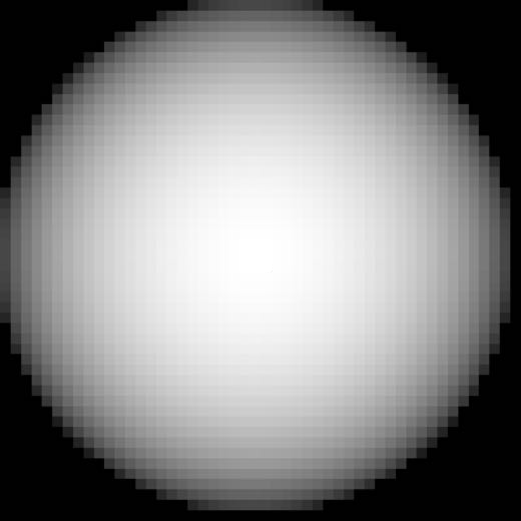
\includegraphics[height=0.1\textwidth]{figures/result/light9.pdf}}
\end{equation*}
The ball on the right represents the light direction. 
Then, in order to reproduce the LED configuration for the proposed RGB ratio model, we define the 3 lighting directions as:
\begin{equation*}
    \begin{split}
        \mathbf{s}_R &= \begin{bmatrix} 0 &0 &-1 &0.15\end{bmatrix}^\top\\
        \mathbf{s}_G &= \begin{bmatrix} 0.3 & 0.2 & -1 & 0.25\end{bmatrix}^\top\\
        \mathbf{s}_B &= \begin{bmatrix} -0.2 & 0.3 & -1 & 0.2\end{bmatrix}^\top\\
    \end{split}
    \qquad\qquad\quad
    \raisebox{-0.7cm}{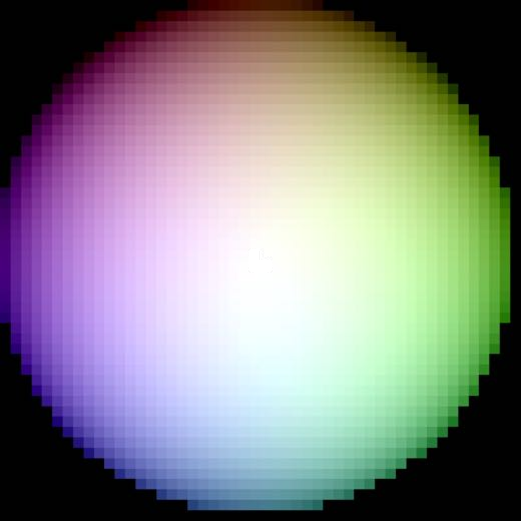
\includegraphics[height=0.1\textwidth]{figures/result/light_color.pdf}}
\end{equation*}
Finally, we need to create a sequence of same images with various directional lights for our robust multi-light model.
A "lighting" matrix $L$ and the corresponding 2D positions (omit the third dimension because they are the same) of 10 point light sources can be illustrated as below, where red points represent the light positions.
\begin{equation*}
\begin{split}
L = 
    \begin{pmatrix}
        0.5 & 0 & -1 & 0.2\\
        0.3 & 0.4 & -1 & 0.2\\
        0 & 0.5 & -1 & 0.2\\
        -0.4 & 0.3 & -1 & 0.2\\
        -0.5 & 0 & -1 & 0.2\\
        -0.3 & -0.4 & -1 & 0.2\\
        0 & -0.5 & -1 & 0.2\\
        0.4 & -0.3 & -1 & 0.2\\
        0 & 0 & -1 & 0.2\\
        0.45 & 0.2 & -1 & 0.2\\
    \end{pmatrix}^\top 
    \qquad 
    &\raisebox{-2.8cm}{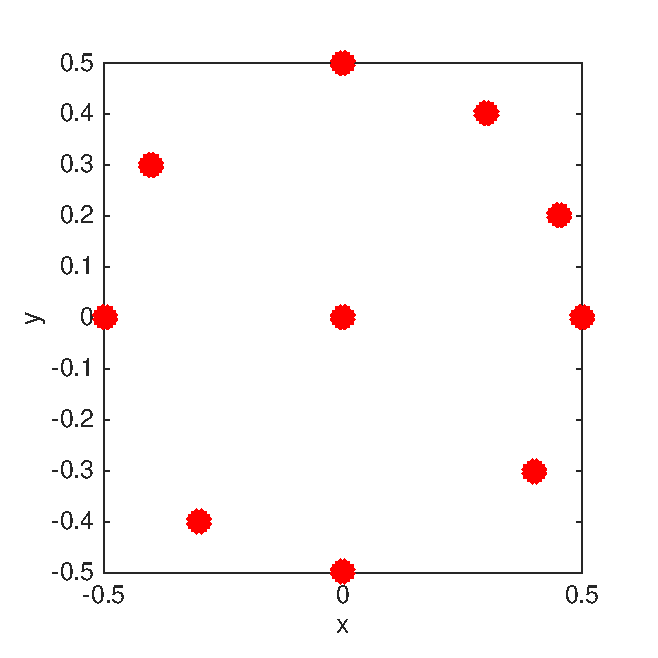
\includegraphics[height=0.4\textwidth]{figures/result/example_multi_light.eps}}\\
    \raisebox{-0.4cm}{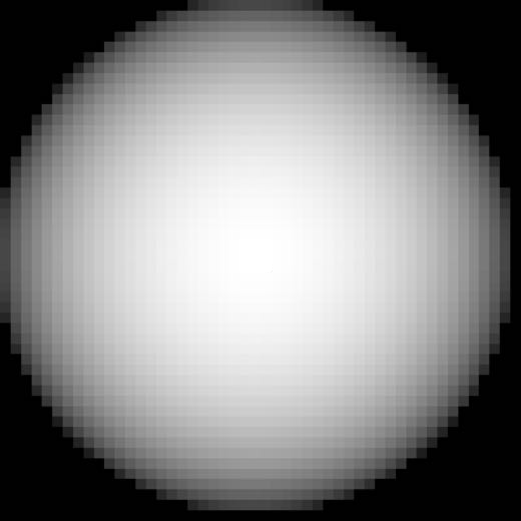
\includegraphics[height=0.1\textwidth]{figures/result/light9.pdf}}    
    \raisebox{-0.4cm}{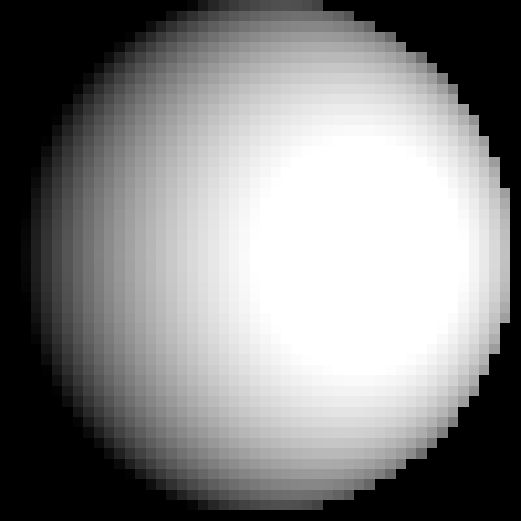
\includegraphics[height=0.1\textwidth]{figures/result/light1.pdf}}
    \raisebox{-0.4cm}{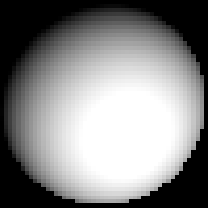
\includegraphics[height=0.1\textwidth]{figures/result/light2.pdf}}
    \raisebox{-0.4cm}{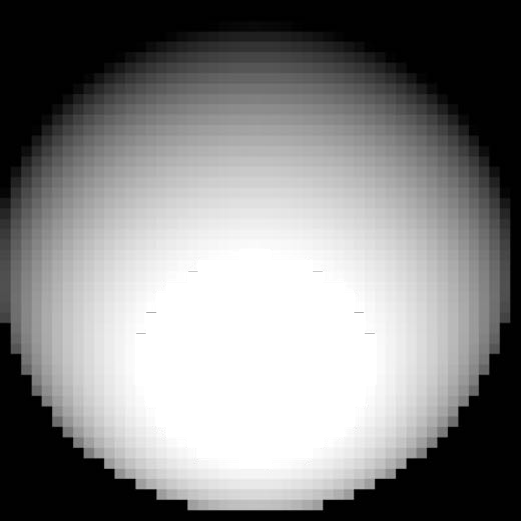
\includegraphics[height=0.1\textwidth]{figures/result/light3.pdf}}
    \raisebox{-0.4cm}{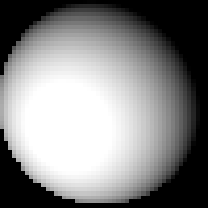
\includegraphics[height=0.1\textwidth]{figures/result/light4.pdf}}
    &\raisebox{-0.4cm}{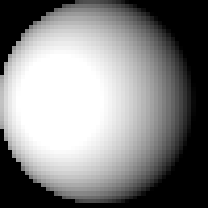
\includegraphics[height=0.1\textwidth]{figures/result/light5.pdf}}
    \raisebox{-0.4cm}{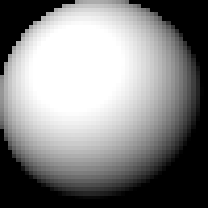
\includegraphics[height=0.1\textwidth]{figures/result/light6.pdf}}
    \raisebox{-0.4cm}{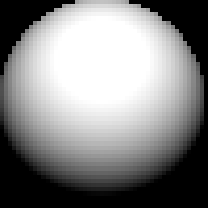
\includegraphics[height=0.1\textwidth]{figures/result/light7.pdf}}
    \raisebox{-0.4cm}{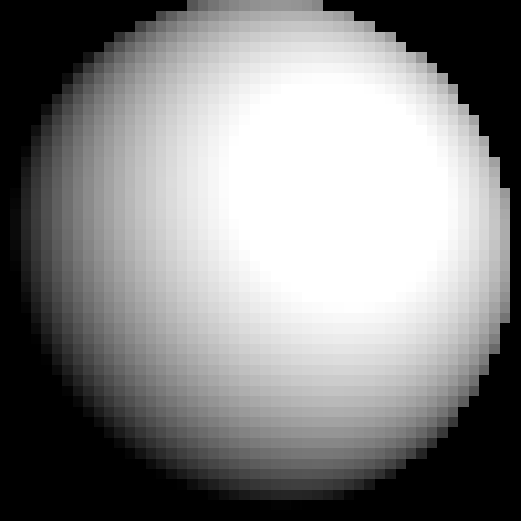
\includegraphics[height=0.1\textwidth]{figures/result/light8.pdf}}
    \raisebox{-0.4cm}{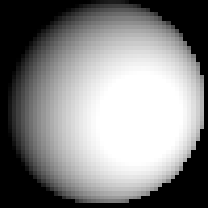
\includegraphics[height=0.1\textwidth]{figures/result/light10.pdf}}
    \end{split}
\end{equation*}
After defining the lighting setup for various methods, three various albedo scenarios  ranging from simple to complicated are listed below:
\begin{itemize}
    \item Red, green and blue piecewise constant areas
    \item Colorful patterns with a few small details inside\footnote{EBSD map. Image courtesy of \url{https://mtex-toolbox.github.io/files/doc/EBSDSpatialPlots.html}}
    \item Colorful patterns with complicated details\footnote{1000 Visual Mashups. Image courtsesy of \url{https://www.flickr.com/photos/qthomasbower/3470650293}}
\end{itemize}
With the albedos and all the pre-defined lights, we can use the Lambertian model mentioned in section~\ref{chap:background} to create the synthetic color images like the first row in Fig.~\ref{fig:result_syn_comp}.


%-------------------------------------------------------------------------------
\subsection{Results Accuracy}
%-------------------------------------------------------------------------------
\textbf{Metrics}
Two metrics have been defined to quantitatively evaluate the performance of depth refinement: root mean square error (RMSE) between ground truth and the estimated depth, and mean angular error (MAE) between the ground truth and estimated normal directions.
We input the rough depth (Fig.~\ref{fig:result_depth}(a)) and obtain the refined depth with various methods and then compare these two metrics with the ground truth, which is shown in Fig.~\ref{fig:result_depth}(b).

Let $z, z_g, N, N_g$ be the input and the ground truth depth as well as their corresponding normals respectively, $m$ the total number of pixels inside the given mask $\mathcal{M}$ and $i$ the index inside the mask, the loose definitions for RMSE and MAE are: 
\begin{align}
    e_{RMSE} &= \sqrt{\frac{\sum\limits_{i}^{m}{(z(i) - z_g(i))^2}}{m}}\\
    e_{MAE} &= \frac{\sum\limits_{i}^{m} \arccos (N(i) \cdot N_g(i))}{m}\label{eq:mae}
\end{align}
The RMSE reflects the global quality of the refined depth (low frequency), while the MAE assesses the precision of the recovered depth (high frequency). 
%It should be mentioned that $e_{MAE}$ in Eq.~\ref{eq:mae} gives values in radians but we convert it to degrees.

\begin{table}[!ht]
\caption{Quantitative evaluations among 4 methods. RMSE and MAE are in millimeters and degrees respectively. ``No smooth'' means no laplacian smoothness term in depth enhancement.}
\vspace{0.5em}
\label{tab:comp_syn_eval}
\centering
\begin{tabular}{lllllll}
                                       & \multicolumn{2}{c}{Simple RGB}                     & \multicolumn{2}{c}{Pattern}                        & \multicolumn{2}{c}{Complicated}            \\\hline
Method                                 & \multicolumn{1}{c}{RMSE} & \multicolumn{1}{c}{MAE} & \multicolumn{1}{c}{RMSE} & \multicolumn{1}{c}{MAE} & \multicolumn{1}{c}{RMSE} & \multicolumn{1}{c}{MAE} \\\hline\hline
Input reference                              & 3.3305                   & 16.3096                 & 3.3305                   & 16.3096                 & 3.3305                   & 16.3096                 \\
RGBD-Fusion\cite{or2015rgbd} (no smooth)                       & 3.3418                   & 18.9115                 & 3.3872                   & 27.0026                 & 3.3411                   & 25.6574          \\
RGBD-Fusion\cite{or2015rgbd} & 3.1751                   & 17.2197                 & 3.1890                   & 18.4722                 & 3.1708                   & 18.0850                 \\ 
Fusion-Like (no smooth)                  & 3.3475                   & 17.5911                 & 3.3459                   & 23.4808                 & 3.3898                   & 35.2610                 \\
Fusion-Like                        & 2.8700                   & 17.1776                 & 2.8749                   & 17.7302                 & 2.8848                   & 19.6452                 \\
RGB ratio model                        & \textbf{1.9437}          & 5.0574         & 2.9116                   & 17.5238                 & 3.1006                   & 21.2286                 \\
Robust multi-light model               & 2.3125                   & \textbf{3.8708}                  & \textbf{1.5794}          & \textbf{1.7368}         & \textbf{1.8424}          & \textbf{2.6815}  \\\hline      
\end{tabular}
\end{table}


According to table~\ref{tab:parameter_setup},~\ref{tab:comp_syn_eval} and Fig.~\ref{fig:result_syn_comp}, there are some interesting observations:
\begin{itemize}
    \item Our RGBD-Fusion Like method uses fewer parameters (5 against 8) and less runtime (7s against 21s) than RGBD-Fusion~\cite{or2015rgbd} but achieves almost the same accuracy.
    \item Adding the Laplacian smoothness term in the depth enhancement energy of RGBD-Fusion method makes a huge improvement on the refined results. In contrast, both our proposed methods have no smoothness term but provide equal or better results.
    \item Single depth image refinement methods (RGBD-Fusion and RGB ratio model) have a chance to acquire satisfactory results only when the albedo is simple with several big color patches. 
    However, they will fail and give even worse results than the input depth in terms of RMSE and MAE when the albedos get complicated. 
    Most of the small details on the albedo of ``Pattern" and ``Complicate Pattern'' cannot be acquired by these methods, which yield the wrong depth estimation with artefacts.
    This is due to the fact that their albedo estimations highly rely on the regularization terms which prefer piecewise smoothness, but this does not meet the condition of most real-world objects.
    \item It can be effortlessly noticed that our robust multi-light method has a strong ability to handle the cases with extremely complicated albedo. 
    Instead of using any regularization terms, our method use only one shading term (Eq.~\ref{eq:robust_albedo_estimate}) to estimate the albedo with extra images illuminated from various light directions. 
    Compared to the albedo estimated by other methods, the albedo from our multi-light method could recover most of the details.
\end{itemize}

\begin{figure}[!ht]
\centering
\setlength{\tabcolsep}{2.2em} % column spacing
 {\renewcommand{\arraystretch}{0.9}% row spacing
\begin{tabular}{c c | c c}
   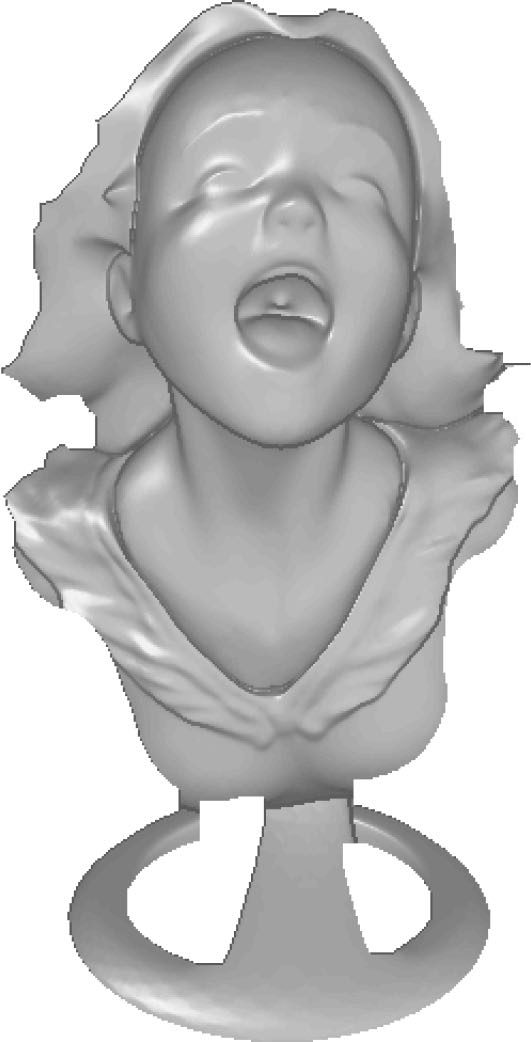
\includegraphics[height = 0.28\linewidth]{figures/result/comp_input_shape.pdf}&
   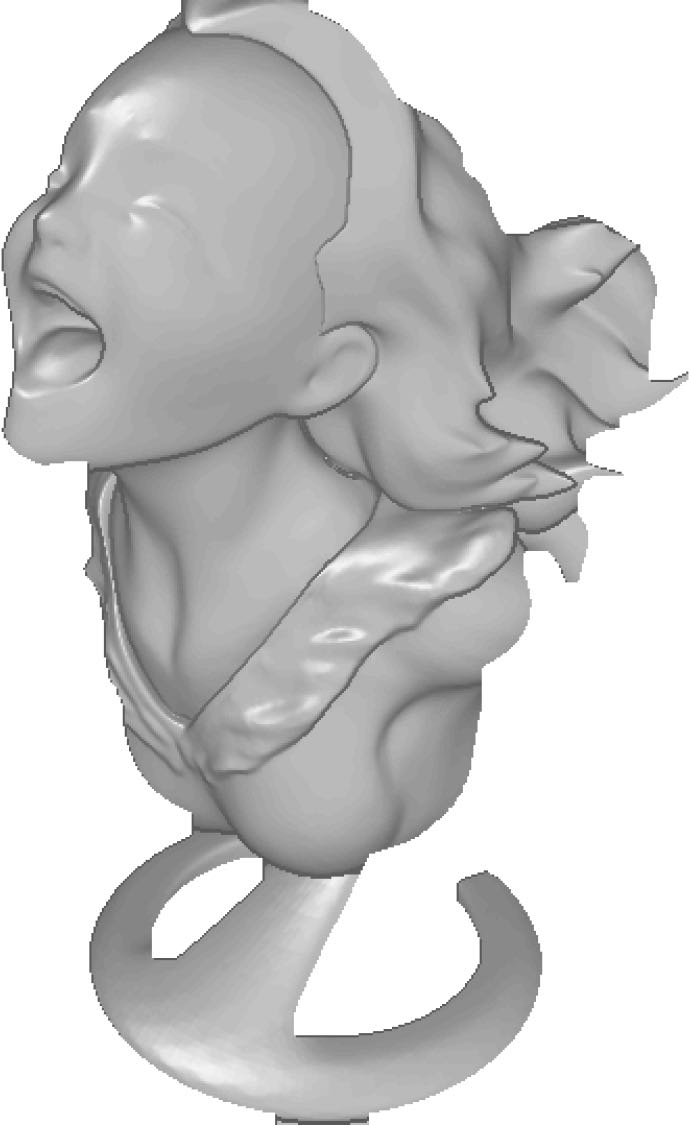
\includegraphics[height = 0.28\linewidth]{figures/result/comp_input_shape_side.pdf}  &
   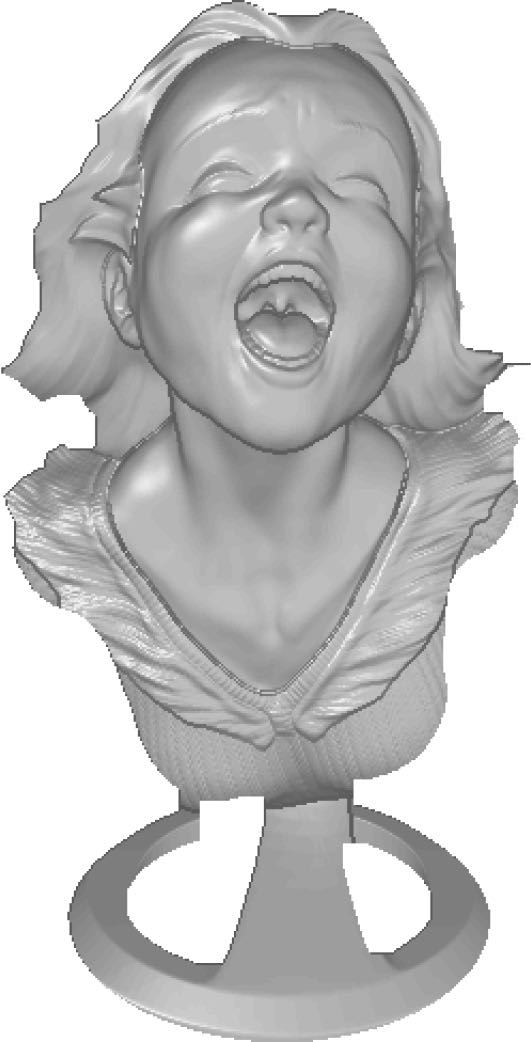
\includegraphics[height = 0.28\linewidth]{figures/result/comp_gt_shape.pdf}  &
   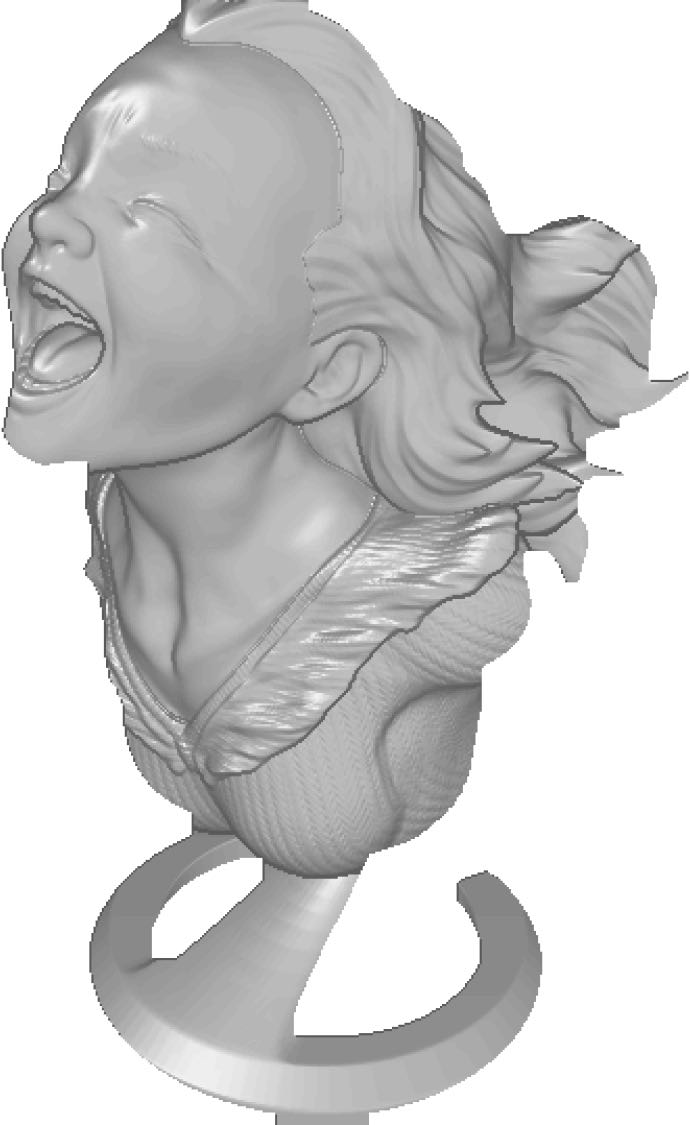
\includegraphics[height = 0.28\linewidth]{figures/result/comp_gt_shape_side.pdf}  \\
\multicolumn{2}{c}{\small (a) Input depth} & \multicolumn{2}{c}{\small (b) Ground truth depth}\\
 \end{tabular}}
\caption{The input depth and the ground truth depth from two views. We only use the cases of frontal direction for the quantitative evaluation, which are the first and the third images.}
\label{fig:result_depth}
\end{figure}
%\begin{figure}[!ht]
%\centering
%\subfigure[Input depth]{\label{fig:result_input_depth}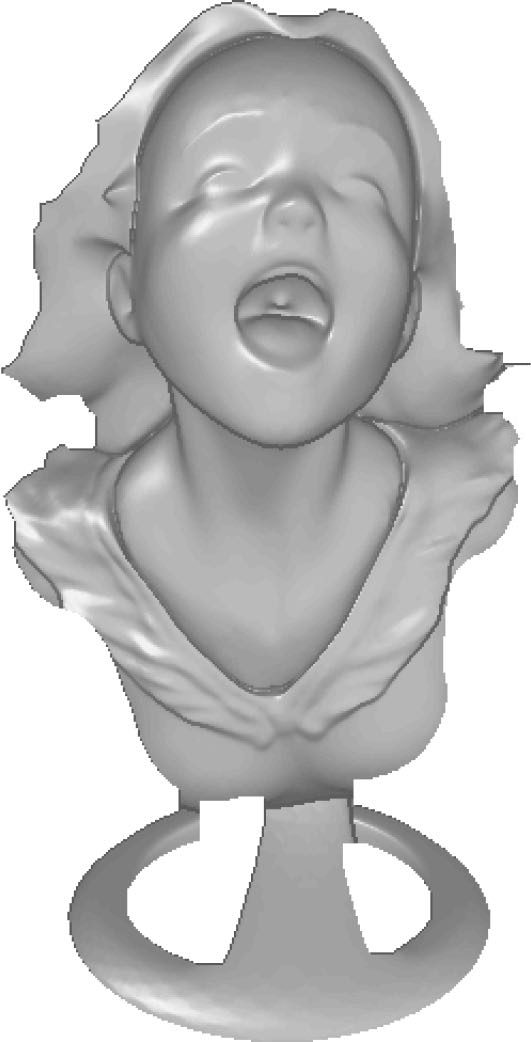
\includegraphics[width=0.13\linewidth]{figures/result/comp_input_shape.pdf}}
%\qquad \qquad
%\subfigure[Ground truth depth]{\label{fig:result_input_depth2}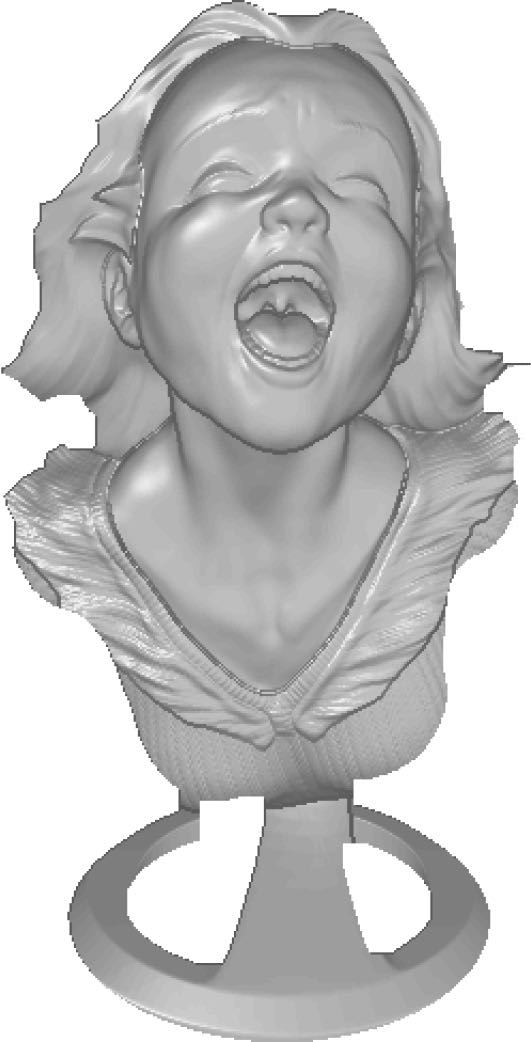
\includegraphics[width=0.13\linewidth]{figures/result/comp_gt_shape.pdf}}
%\caption{The input depth and the ground truth depth for the quantitative evaluation. The errors for the rough input depth are RMSE of 3.35 and MAE of 16.75.}
%\label{fig:comp_syn_input}
%\end{figure}
\begin{figure}[H]
  % Top row: Ground truth, Image + SH, Image + SH, Image + SH
  \setlength{\tabcolsep}{0.5em} % for the horizontal padding
{\renewcommand{\arraystretch}{0.6}% for the vertical padding
\begin{tabular}{cccc}
%    \multicolumn{2}{c}{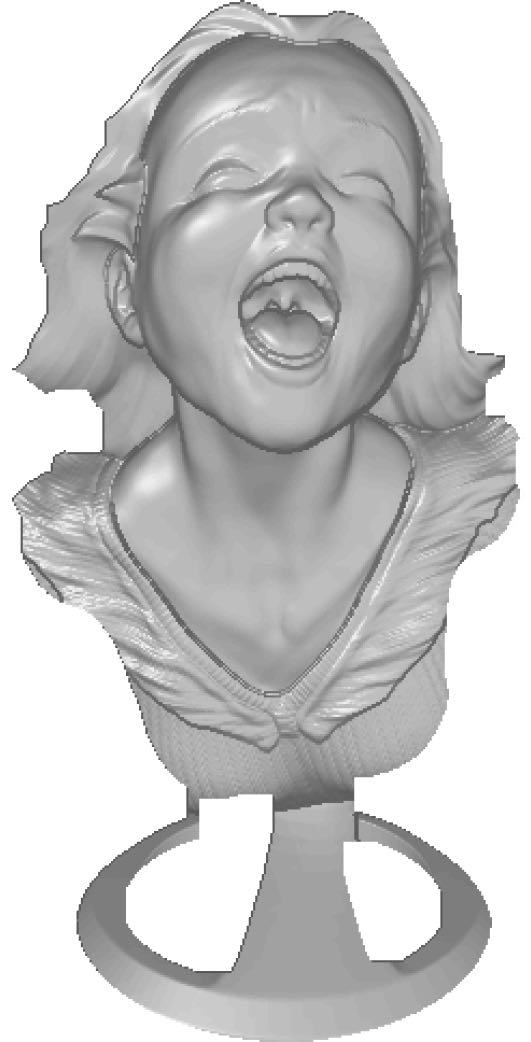
\includegraphics[width=0.1\linewidth]{figures/result/comp_robust_pattern_shape.pdf}} &
&
    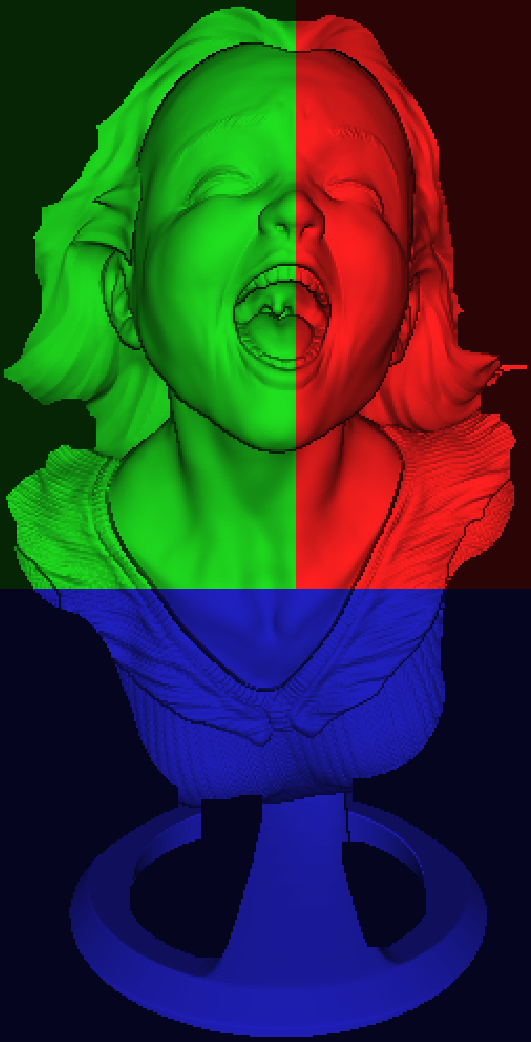
\includegraphics[height=0.25\linewidth]{figures/result/comp_simple_rgb.pdf}
    
\includegraphics[height=0.25\linewidth]{figures/result/comp_simple_albedo.pdf}& 
    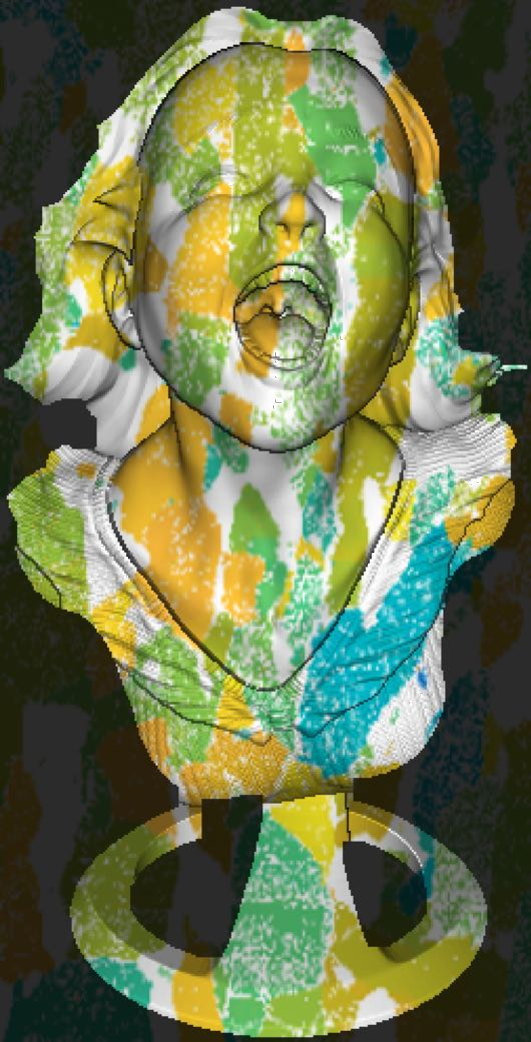
\includegraphics[height=0.25\linewidth]{figures/result/comp_pattern_rgb.pdf} 
    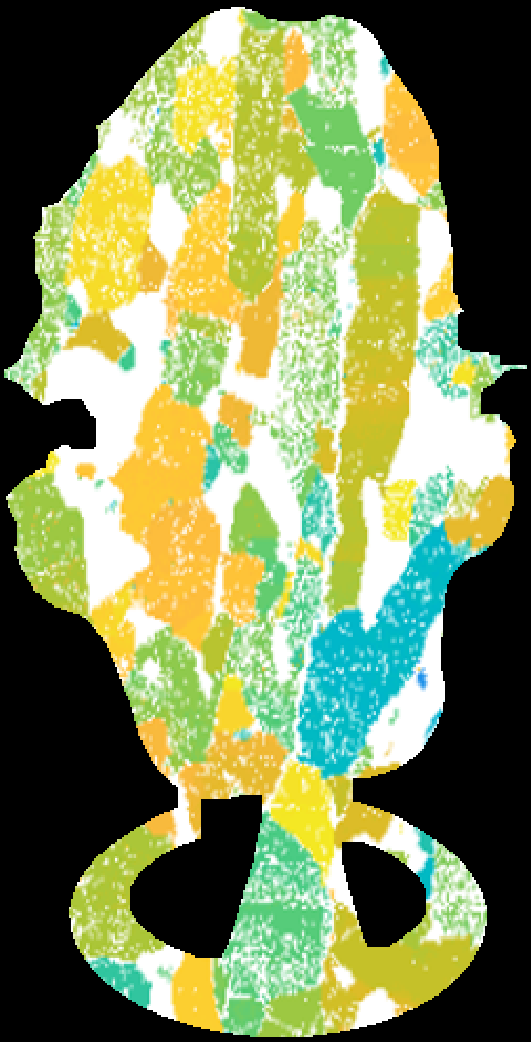
\includegraphics[height=0.25\linewidth]{figures/result/comp_pattern_albedo.pdf}& 
    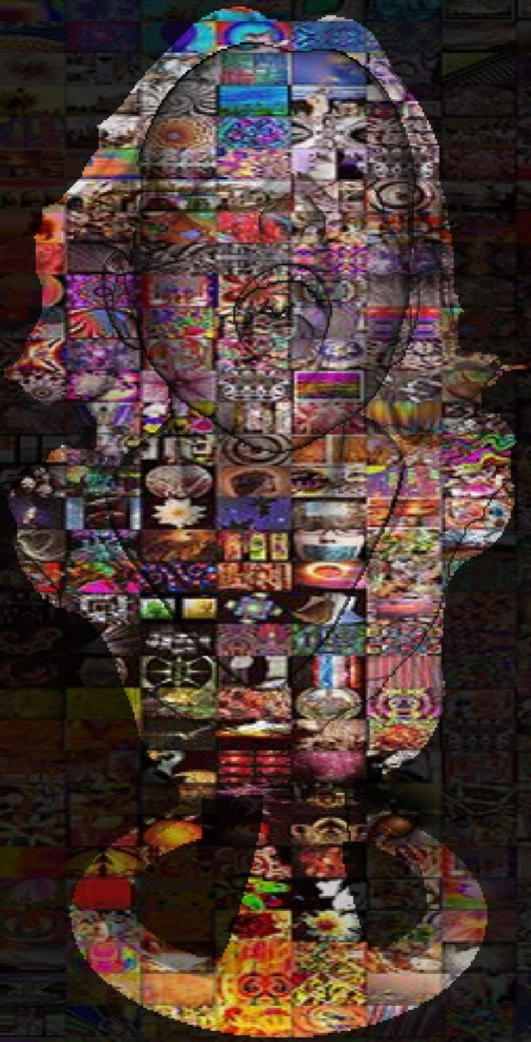
\includegraphics[height=0.25\linewidth]{figures/result/comp_love_rgb.pdf}
    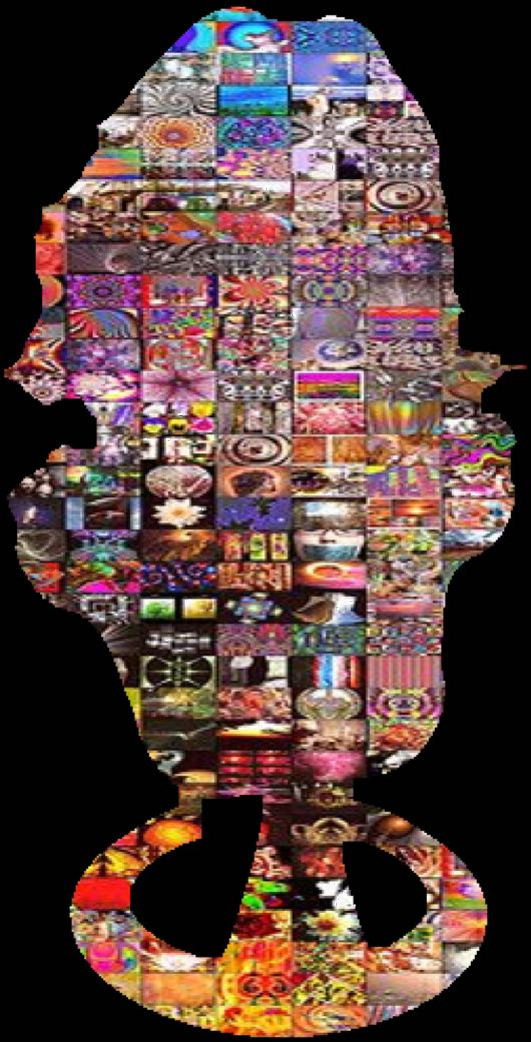
\includegraphics[height=0.25\linewidth]{figures/result/comp_love_albedo.pdf} \\
% \multicolumn{2}{c}{ {\small Ground truth}}  &
     & {\small Simple RGB} & {\small Pattern} & {\small Complicated Pattern } \\
%%%%%%%%%%%%%%%%%%%%%%%%%%%%%%%%%%%%%%%%%%%%%%%%%%%% 
  % Initial guess
  
%  \multirow{2}{*}{
%  \begin{tabular}{c}
%  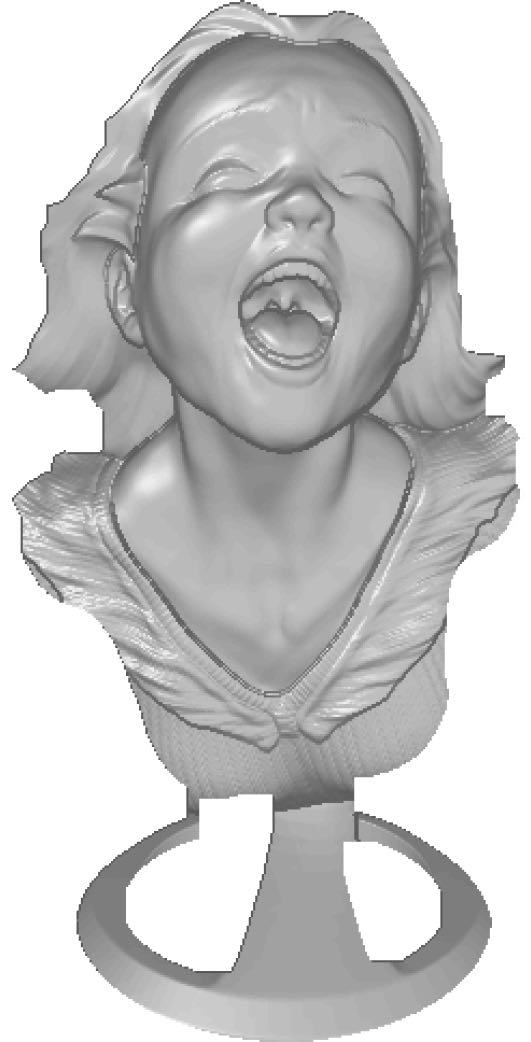
\includegraphics[width=0.1\linewidth]{figures/result/comp_robust_pattern_shape.pdf} \\ Non-realistic \\ initialization 
%  \end{tabular}} &

  % RGBD-Fusion without smoothing
  % Simple RGB
\multirow{-15}{*}{\parbox[t]{2.5mm}{\rotatebox[origin=c]{90}{\small RGBD-Fusion~\cite{or2015rgbd} $\lambda_l = 0$}}} &
 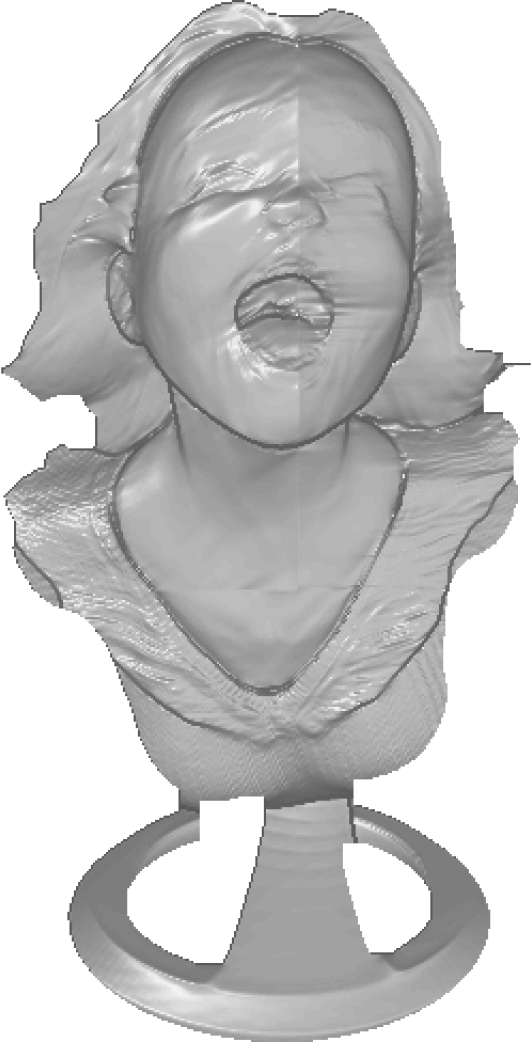
\includegraphics[height=0.25\linewidth]{figures/result/comp_fusion_rgbN_shape.pdf}
 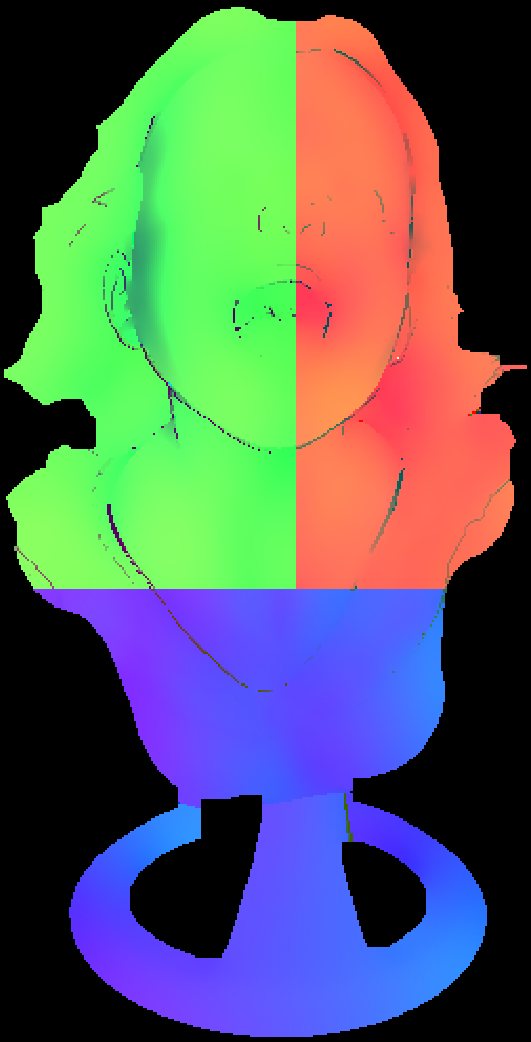
\includegraphics[height=0.25\linewidth]{figures/result/comp_fusion_rgbN_albedo.pdf} &
  % Pattern
 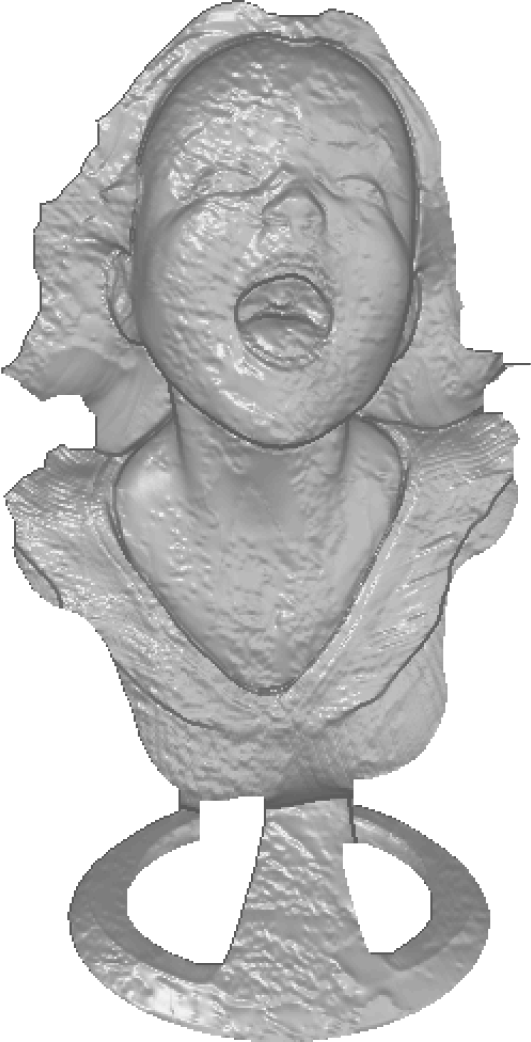
\includegraphics[height=0.25\linewidth]{figures/result/comp_fusion_patternN_shape.pdf} 
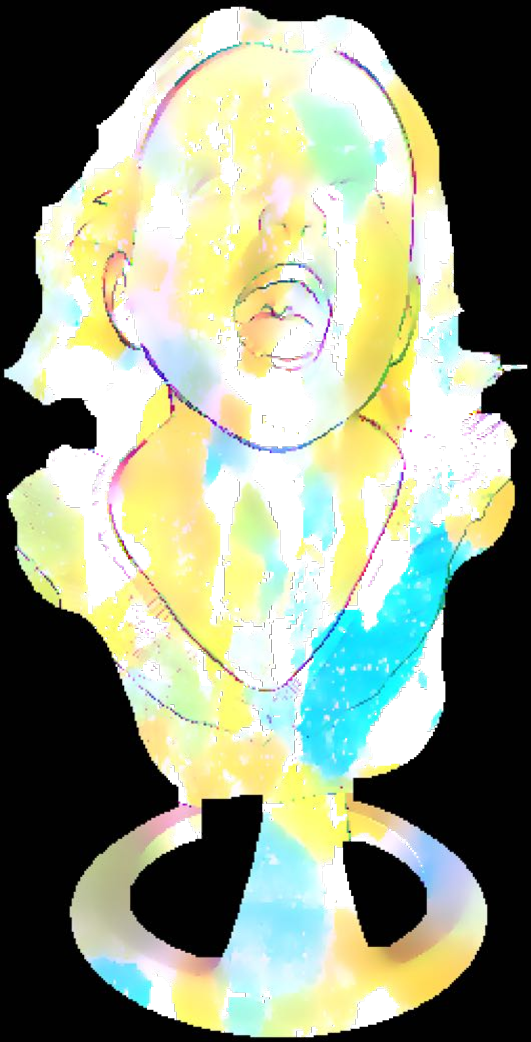
\includegraphics[height=0.25\linewidth]{figures/result/comp_fusion_patternN_albedo.pdf} &
  % Complicate Pattern
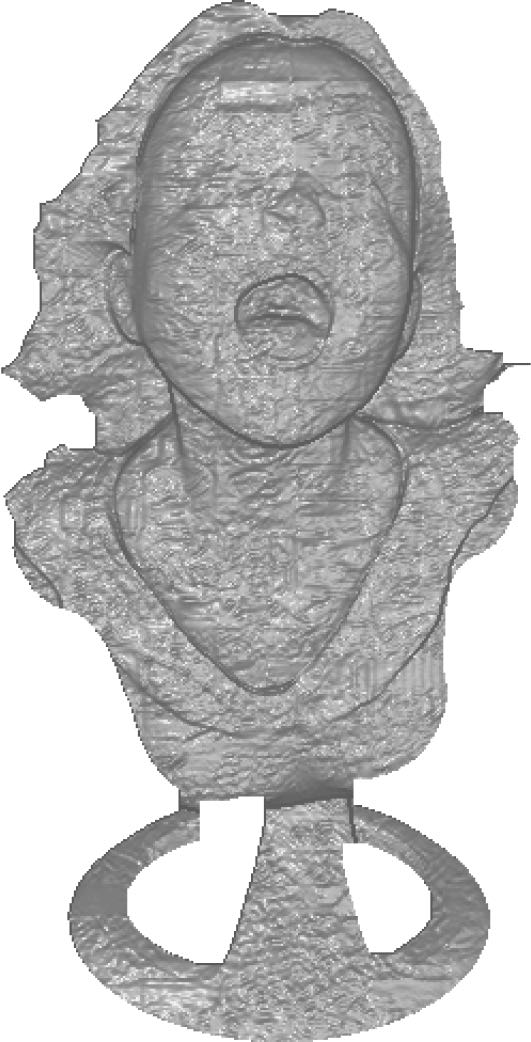
\includegraphics[height=0.25\linewidth]{figures/result/comp_fusion_loveN_shape.pdf} 
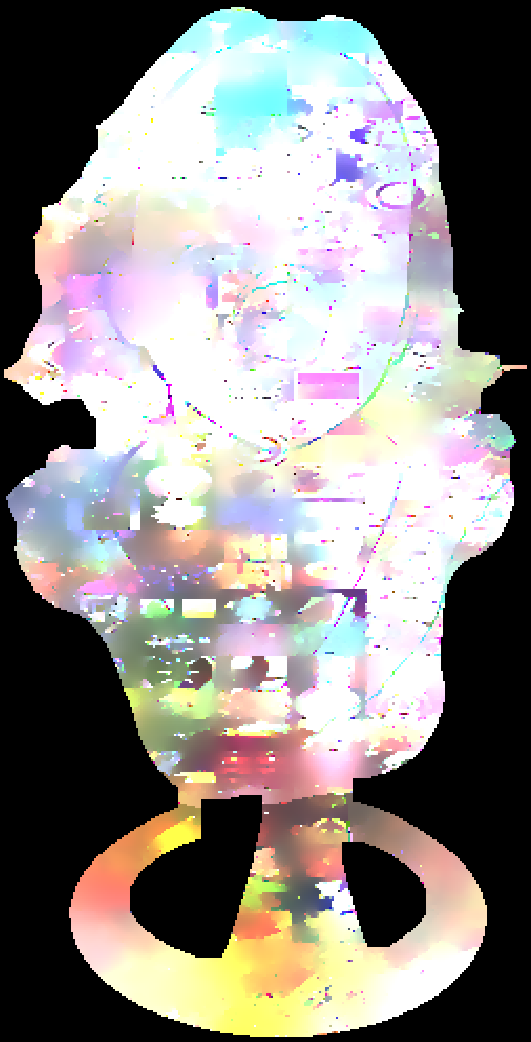
\includegraphics[height=0.25\linewidth]{figures/result/comp_fusion_loveN_albedo.pdf} \\
& {\small RMSE $= 3.35$, MAE $=17.60$} & {\small RMSE $= 3.35$, MAE $=23.48$} & {\small RMSE $= 3.39$, MAE $=35.26$} \\
%%%%%%%%%%%%%%%%%%
  % {\small Non-realistic initial guess} & % Same for SIRFS
  % Ours - Dir
\multirow{-15}{*}{\parbox[t]{2.5mm}{\rotatebox[origin=c]{90}{\small RGBD-Fusion~\cite{or2015rgbd}}}}&
 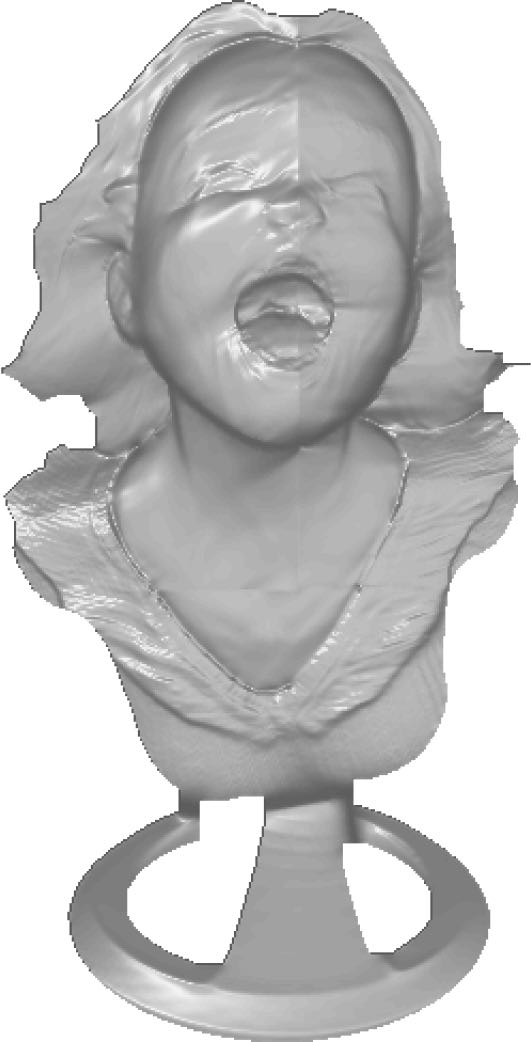
\includegraphics[height=0.25\linewidth]{figures/result/comp_fusion_rgb_shape.pdf}
 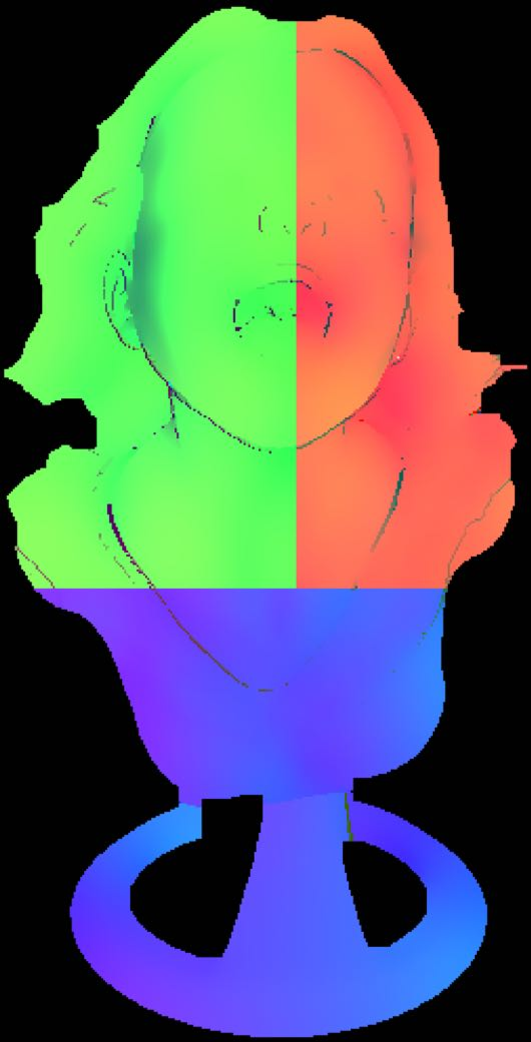
\includegraphics[height=0.25\linewidth]{figures/result/comp_fusion_rgb_albedo.pdf} &
  % Ours - SH2
 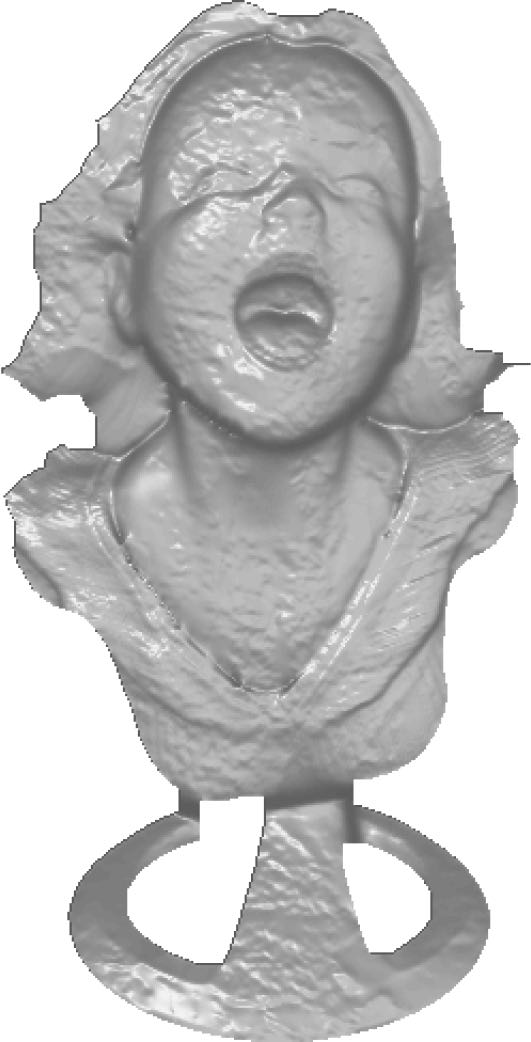
\includegraphics[height=0.25\linewidth]{figures/result/comp_fusion_pattern_shape.pdf} 
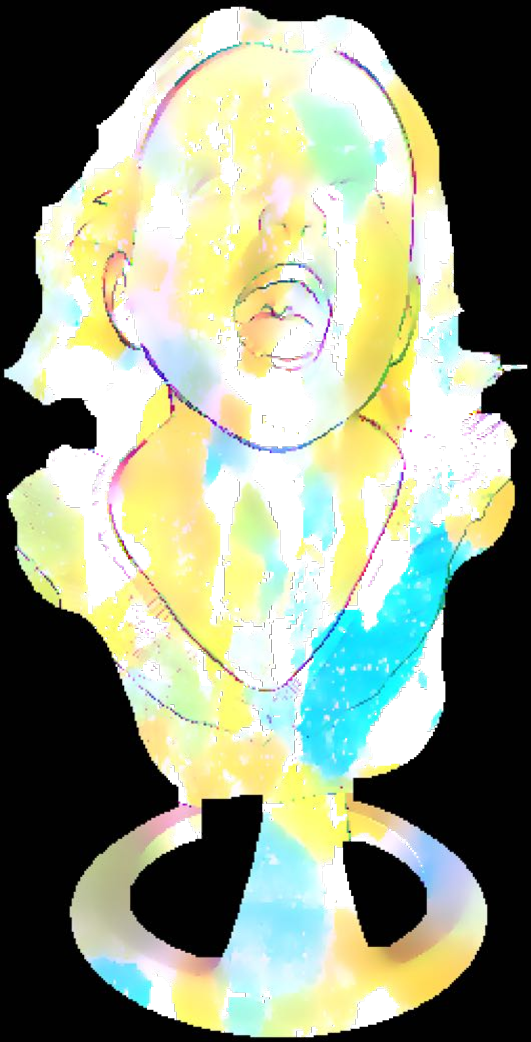
\includegraphics[height=0.25\linewidth]{figures/result/comp_fusion_pattern_albedo.pdf} &
  % Ours - SH2 color
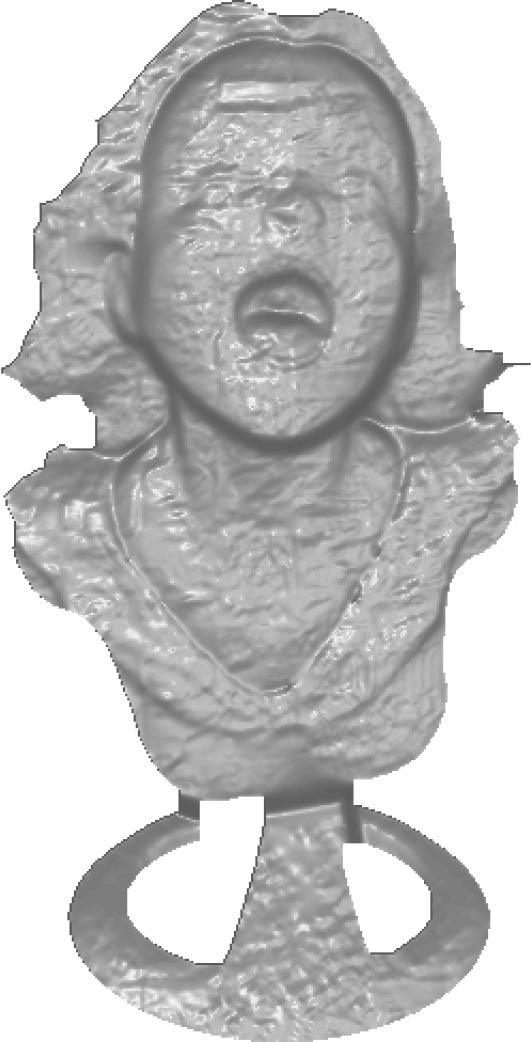
\includegraphics[height=0.25\linewidth]{figures/result/comp_fusion_love_shape.pdf} 
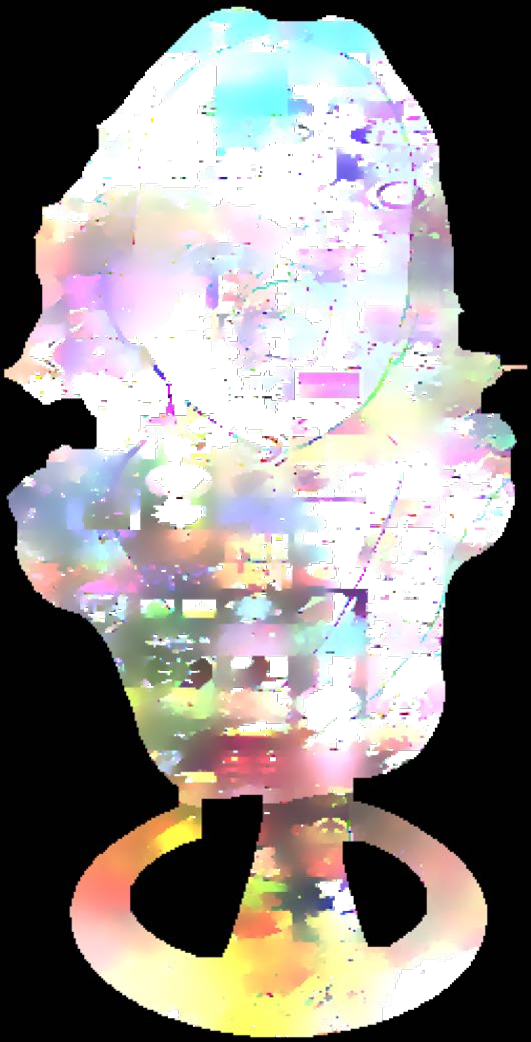
\includegraphics[height=0.25\linewidth]{figures/result/comp_fusion_love_albedo.pdf} \\
& {\small RMSE $= 2.87$, MAE $=17.17$} & {\small RMSE $= 2.88$, MAE $=17.73$} & {\small RMSE $=2.89$, MAE $=19.64$} \\
%%%%%%%%%%%%%%%%%%%%%%%%%%%%%%%%%%%%%%%%%%%%%%%%%%%%
% \multirow{2}{*}{
% \begin{tabular}{c}
%  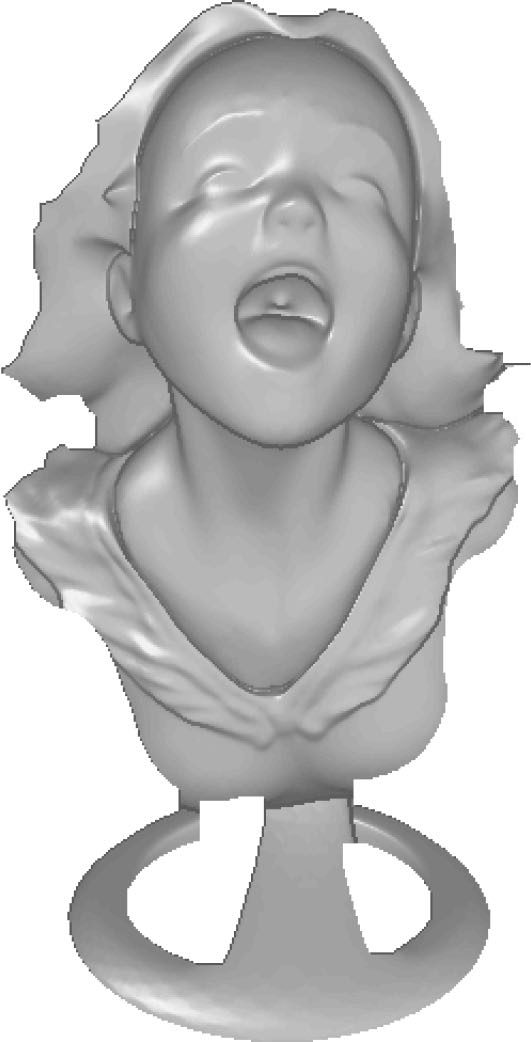
\includegraphics[width=0.1\linewidth]{figures/result/comp_input_shape.pdf} \\
%  Realistic \\
%   initialization \end{tabular}} &

\multirow{-15}{*}{\parbox[t]{2.5mm}{\rotatebox[origin=c]{90}{\small RGB Ratio}}} &    
 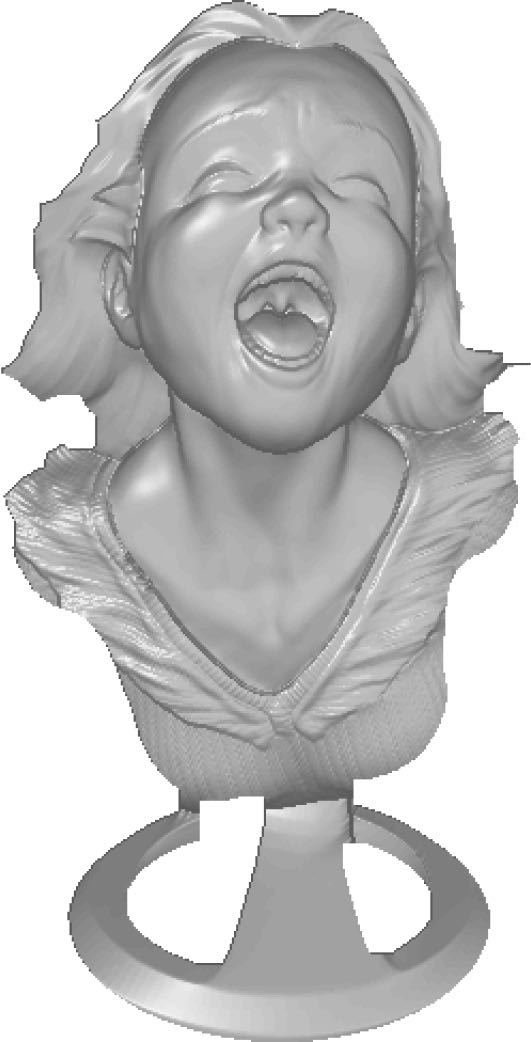
\includegraphics[height=0.25\linewidth]{figures/result/comp_ratio_rgb_shape.pdf}
 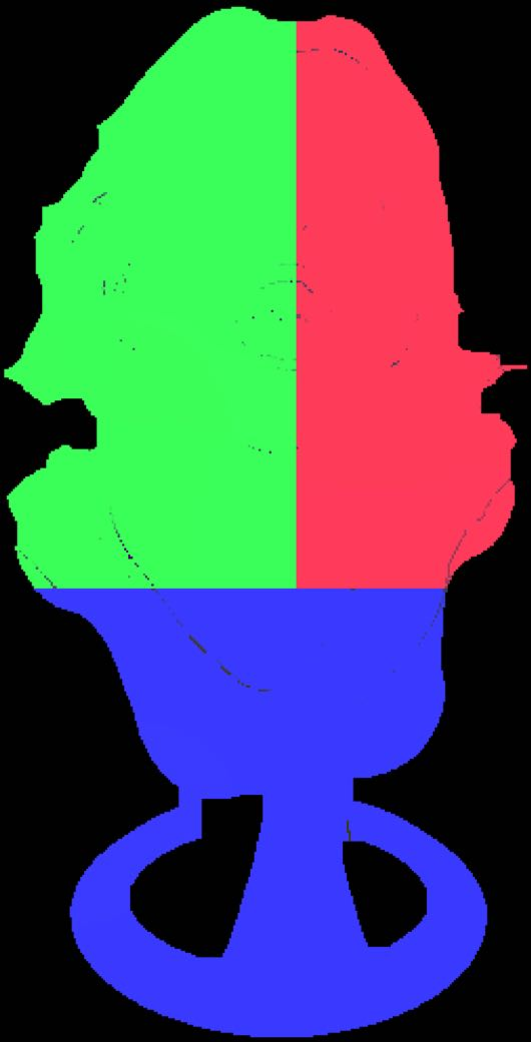
\includegraphics[height=0.25\linewidth]{figures/result/comp_ratio_rgb_albedo.pdf} &
  % Pattern
 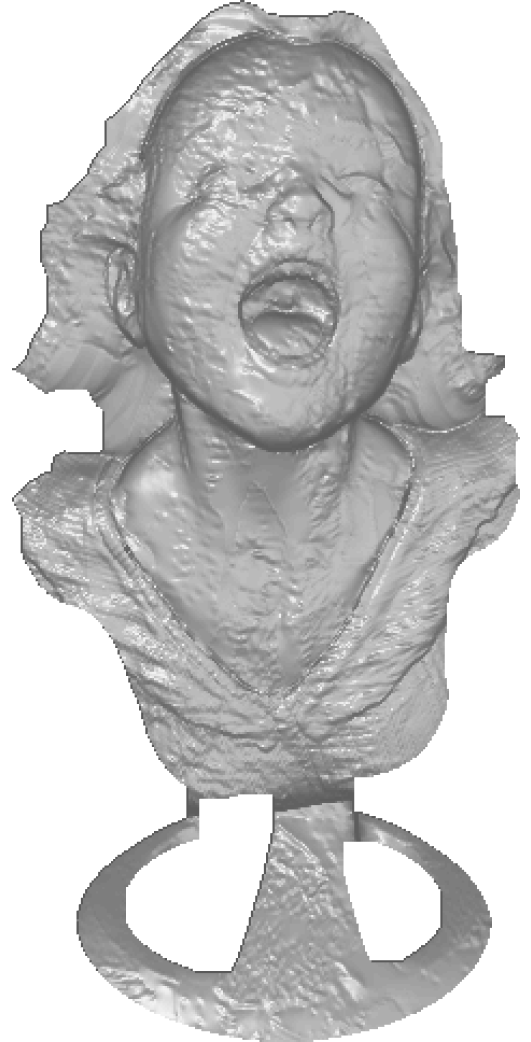
\includegraphics[height=0.25\linewidth]{figures/result/comp_ratio_pattern_shape.pdf} 
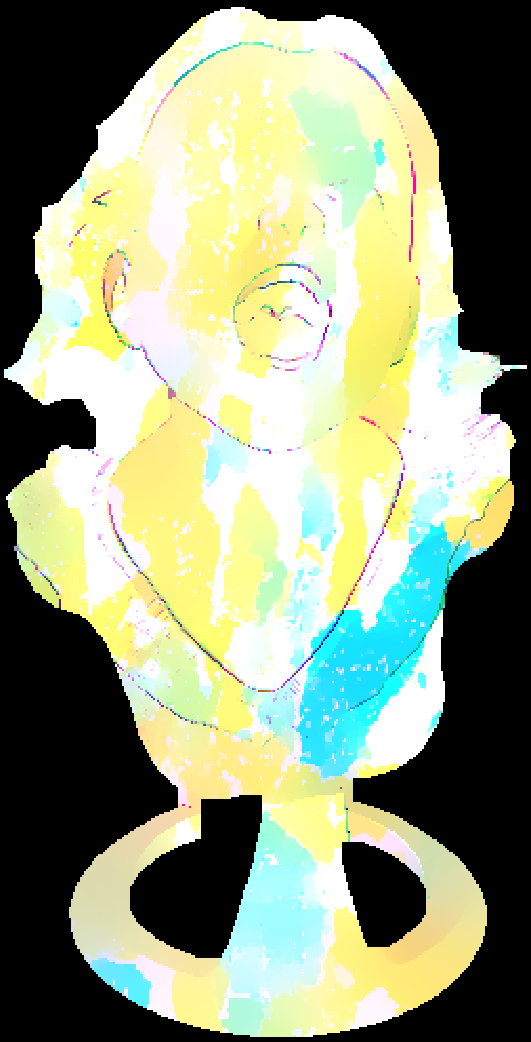
\includegraphics[height=0.25\linewidth]{figures/result/comp_ratio_pattern_albedo.pdf} &
  % Complicate Pattern
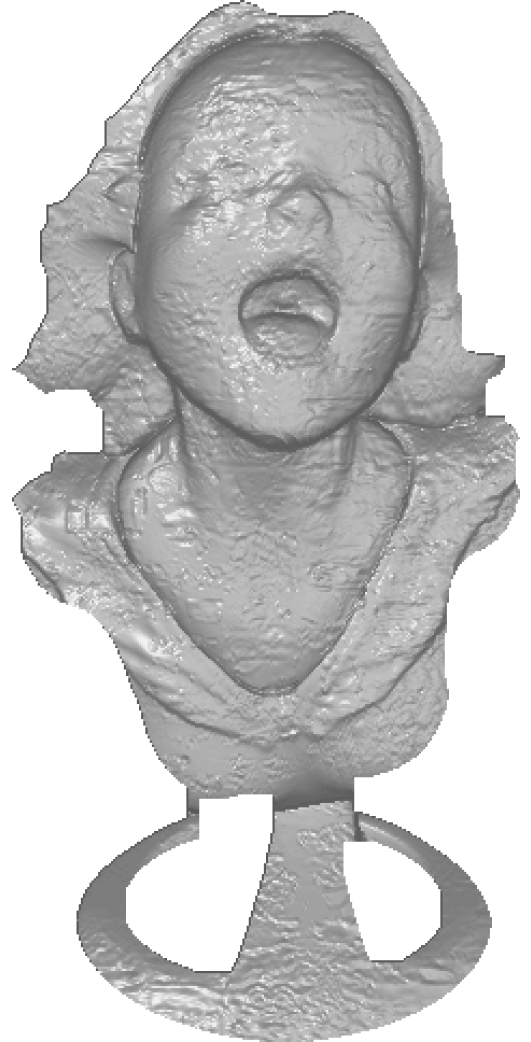
\includegraphics[height=0.25\linewidth]{figures/result/comp_ratio_love_shape.pdf} 
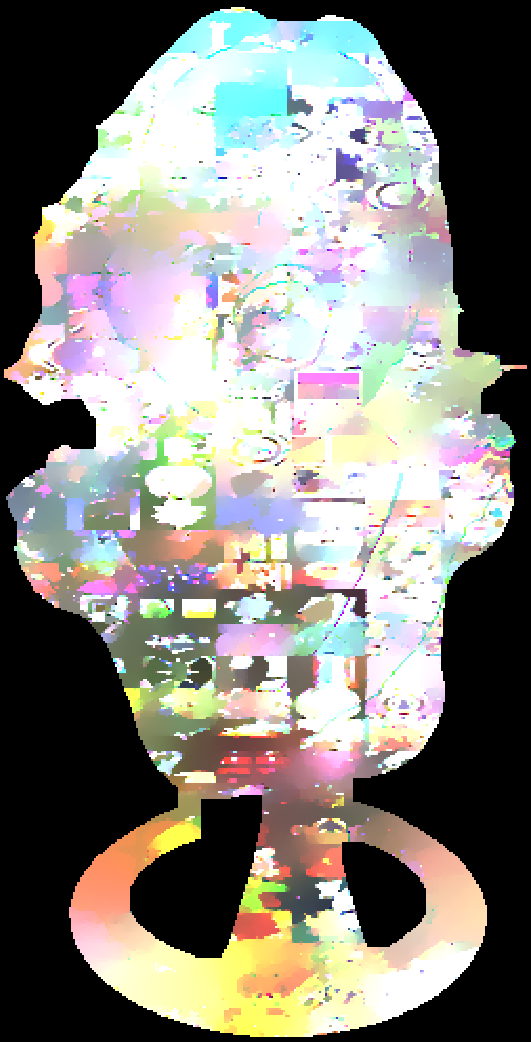
\includegraphics[height=0.25\linewidth]{figures/result/comp_ratio_love_albedo.pdf} \\
& {\small RMSE $= \textbf{1.94}$, MAE $=5.06$} & {\small RMSE $= 2.91$, MAE $=17.52$} & {\small RMSE $= 3.10$, MAE $=21.22$} \\
%%%%%%%%%%%%%%%%%%

\multirow{-15}{*}{\parbox[t]{2.5mm}{\rotatebox[origin=c]{90}{\small Multi-Light}}} &   
 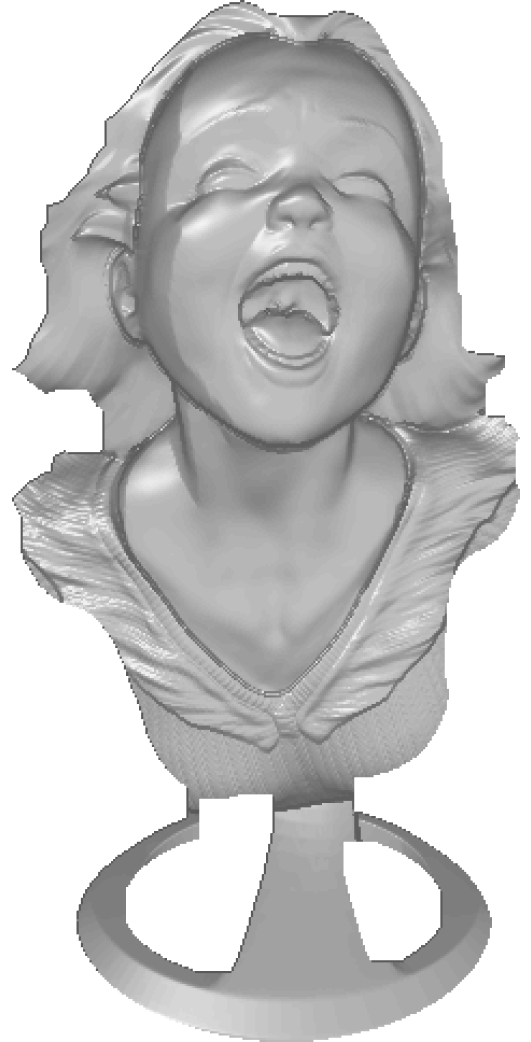
\includegraphics[height=0.25\linewidth]{figures/result/comp_robust_rgb_shape.pdf}
 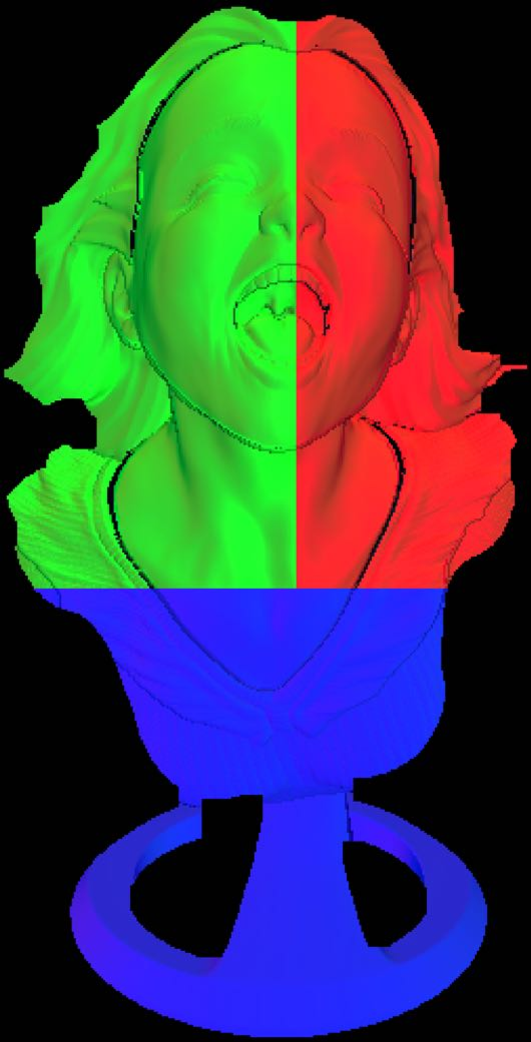
\includegraphics[height=0.25\linewidth]{figures/result/comp_robust_rgb_albedo.pdf} &
  % Pattern
 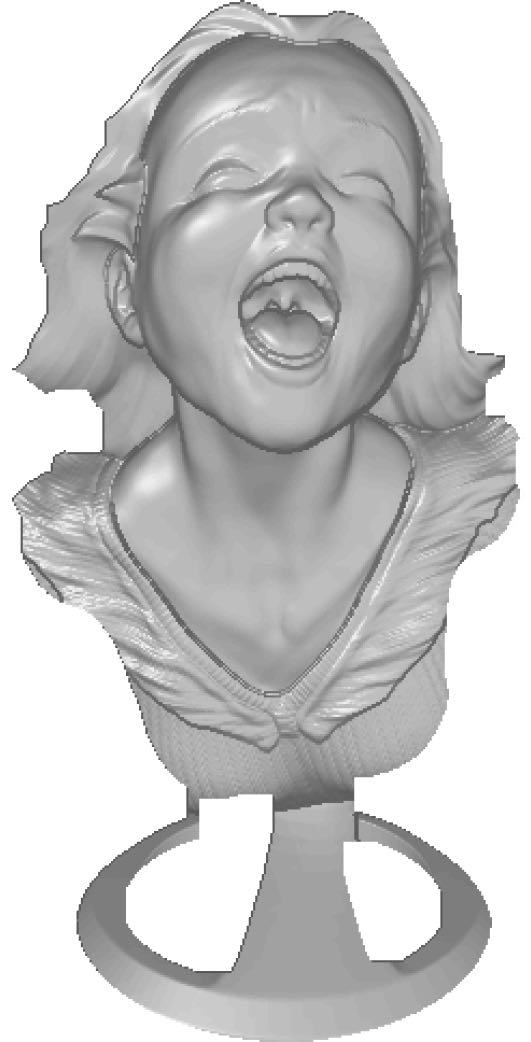
\includegraphics[height=0.25\linewidth]{figures/result/comp_robust_pattern_shape.pdf} 
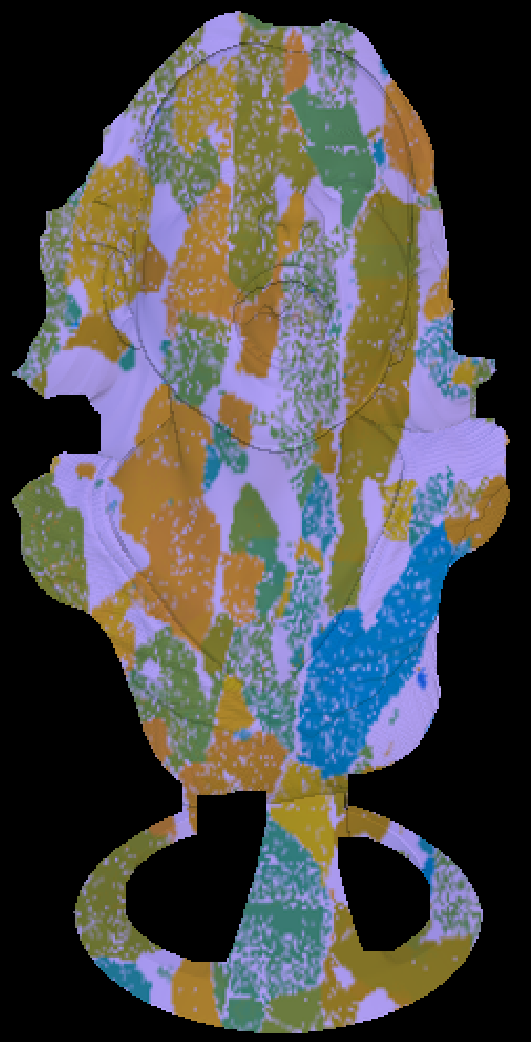
\includegraphics[height=0.25\linewidth]{figures/result/comp_robust_pattern_albedo.pdf} &
  % Complicate Pattern
\includegraphics[height=0.25\linewidth]{figures/result/comp_robust_love_shape.pdf} 
\includegraphics[height=0.25\linewidth]{figures/result/comp_robust_love_albedo.pdf} \\
& {\small RMSE $= 2.32$, MAE $=\textbf{3.87}$} & {\small RMSE $= \textbf{1.58}$, MAE $=\textbf{1.73}$} & {\small RMSE $= \textbf{1.84}$, MAE $=\textbf{2.68}$} \\
 \\
%%%%%%%%%%%%%%%%%%%%%%%%%%%%%%%%%%%%%%%%%%%%%%%%%%%%
  \end{tabular}
  }
  \caption{Evaluation of our two proposed methods RGB ratio model and robust multi-light method against the RGBD-Fusion~\cite{or2015rgbd}, under three albedos scenarios from simple to complicated. The first row is the input color images and their ground truth albedos, while the rest are the estimated depths and albedos using the parameters defined in table~\ref{tab:parameter_setup}. The errors for the rough input depth are RMSE of 3.33 and MAE of 16.30. Our proposed methods can deal with the complicated albedo and outperform RGBD-Fusion in all tests.}
  \label{fig:result_syn_comp}
\end{figure}


%-------------------------------------------------------------------------------
\subsection{Runtime}
%-------------------------------------------------------------------------------
First of all, all the tests are performed in MATLAB R2015b under Mac OSX 10.10.5, Intel Core i5 2.7GHz, 2 cores, 8GB memory. 
The resolution of our synthetic image is $540\times 960$.

We first compare the runtime for 4 methods, which is shown in table~\ref{tab:runtime}.
It is noticeable that our implementation of RGBD-Fusion like method is much faster than the original approach while the accuracy from our implementation is quite similar to the original one.
On the one hand, we only consider the pixel inside the mask while the official implementation\footnote{Source code of official RGBD-Fusion implementation can be found: \url{https://cs.technion.ac.il/~royorel/rgbd_fusion.html}} uses the whole image.
On the other hand, instead of estimating the ambient light for each pixel with an extra energy, we directly treat the ambient light as one parameter inside the first-order spherical harmonics so the ambient light could be obtained along with lighting directions.

It should be mentioned that both our proposed approaches are indeed about twice slower than RGBD-Fusion method. 
However, the RGBD-Fusion method stops when the overall energy starts increasing, which happens merely in $1-3$ iterations based on our experiment.  
In contrast, the minimization for our methods are both convergent so the runtime highly relies on the threshold for the relative change of the energy values.

\begin{table}[!ht]
\caption{The comparison of the runtime among RGBD-Fusion method, our implementation RGBD-Fusion Like method,  proposed RGB ratio model and robust multi-light method in synthetic data.}
\label{tab:runtime}
\centering
\begin{tabular}{|m{4cm} |m{7cm}|}
\hline
\multicolumn{1}{|c|}{Method}                               & \multicolumn{1}{c|}{Runtime (s)}                                                                                                                 \\ \hline
RGBD-Fusion~\cite{or2015rgbd} & \multicolumn{1}{c|}{21.64}             \\ \hline
RGBD-Fusion Like                     & \multicolumn{1}{c|}{7.75}      \\ \hline
Proposed I: RGB Ratio                            & \multicolumn{1}{c|}{49.33}        \\ \hline
Proposed II: Multi-Light                        & \multicolumn{1}{c|}{52.82}\\ \hline
\end{tabular}
\end{table}

Now for the proposed robust multi-light method, we are interested in understanding how the number of different illuminations makes the difference in the runtime as well as the RMSE and MAE.
To perform the experiment, we randomly pre-defined 40 illumination directions and constructed the corresponding synthetic color images as discussed in section~\ref{sec:synthetic}.

%And then we picked $3,6,10,15,20,30, 40$ images from this new dataset and recorded the runtime in each iteration as well as the final errors when the stopping criteria in Alg.~\ref{alg:robust} set to $\epsilon = 0.01$.

It has been shown in Fig.~\ref{fig:result_runtime} that when the number of images increases, the runtime for each iteration has linearly ascent, while two errors decrease and reach a platform. 
This is reasonable because the details on a certain part of the object can be retrieved when there exists light on it. 
Therefore, the more various lightings we have, the more details we can obtain.
If we take the comprehensive consideration, $10\sim20$ would be the suitable number for illuminations.

\begin{figure}[!ht]
    \centering
    \includegraphics[height = 0.6\linewidth]{figures/result/runtime.eps} 
    \caption{Illustrations for the runtime, RMSE and MAE in various number of illuminations for the proposed robust multi-light method. $10\sim20$ is the suitable number for different lightings.}
\label{fig:result_runtime}
\end{figure}


%%%%%%%%%%%%%%%%%%%%%%%%%%%%%%%%%%%%%%%%%%%%
\section{Qualitative Evaluation}
%----------------------------------------------
Except for the quantitative evaluation, we have found out that our robust multi-light method also outperforms the state-of-the-art methods qualitatively in many aspects.
In this part, we will first show the robustness of depth estimation of the proposed multi-light method on the objects with complicated albedo.
Then, we will demonstrate the performance on the specular (non-Lambertian) objects.
In addition, as mentioned in chapter~\ref{chap:background}, uncalibrated photometric stereo suffers from the GBR ambiguity.
So we will finally exemplify that our method also outperforms other photometric stereo algorithms because of the input depth cues.

%----------------------------------------------
\subsection{Complicated albedo objects}
%----------------------------------------------
It has already been illustrated in Fig.~\ref{fig:result_syn_comp} that our robust multi-light method has the capability of acquiring the shape of synthetic objects with very complex albedo.
In contrast, the state-of-the-art depth enhancement methods with one image work well for many simple color objects, but could not separate the complicated albedo from the real shape of the object, which leads to severe artefacts on the final estimated depth. 
Figure~\ref{fig:comp_complicated_albedo} has proved that this judgment still holds correct for the real-world objects.
To be fair, we set the parameter for Laplacian smoothness term in RGBD-Fusion to zero.

%&&&&&&&&&&&&&&&&&&&&&&&&&
%\begin{figure}[!ht]
%\centering
%\setlength{\tabcolsep}{0.1em} % column spacing
% {\renewcommand{\arraystretch}{3.2}% row spacing
%\begin{tabular}{c|c c c}
%   \includegraphics[height = 0.21\linewidth]{figures/result/robust_padback_rgb2.pdf} 
%   &
%   \includegraphics[height = 0.21\linewidth]{figures/result/rgbd_padback_normal_detail.pdf} &
%   \includegraphics[height = 0.21\linewidth]{figures/result/robust_padback_normal_detail.pdf}&
%      \parbox[b]{1.5cm}{
%   \includegraphics[width=0.105\textwidth]{figures/result/rgbd_padback_normal_crop.png}\\
%   \includegraphics[width=0.105\textwidth]{figures/result/robust_padback_normal_crop.png}} 
%   \\
%
%   \includegraphics[height = 0.21\linewidth]{figures/result/robust_padback_shape_init.pdf} 
%   &
%   \includegraphics[height = 0.21\linewidth]{figures/result/rgbd_padback_shape.pdf} &
%   \includegraphics[height = 0.21\linewidth]{figures/result/robust_padback_shape.pdf}
%   &
%   \\
%\hline
%   \includegraphics[height = 0.21\linewidth]{figures/result/robust_patternShirt_rgb.pdf} 
%   &
%   \includegraphics[height = 0.21\linewidth]{figures/result/rgbd_patternShirt_normal_detail.pdf} &
%   \includegraphics[height = 0.21\linewidth]{figures/result/robust_patternShirt_normal_detail.pdf}&
%   \parbox[b]{1.5cm}{
%   \includegraphics[width=0.105\textwidth]{figures/result/rgbd_patternShirt_normal_crop.png}\\
%   \includegraphics[width=0.105\textwidth]{figures/result/robust_patternShirt_normal_crop.png}}
%    \\
%   \includegraphics[height = 0.21\linewidth]{figures/result/robust_patternShirt_shape_init.pdf} 
%   &
%   \includegraphics[height = 0.21\linewidth]{figures/result/rgbd_patternShirt_shape.pdf} &
%   \includegraphics[height = 0.21\linewidth]{figures/result/robust_patternShirt_shape.pdf}
%   &
%   \vspace{-2em}
%   \\
%   {Input} & {RGBD-Fusion~\cite{or2015rgbd}} & {Proposed Multi-Light Model}  &{}             \\
% \end{tabular}}
%\caption{Comparisons between our multi-light model and RGBD-Fusion for two specular objects. On the first column, the RGB images of the iPad cover and the shirt are ones of the 10 various illuminations. The first and third rows correspond to the surface normals, while the second and fourth are the refined depths. Our method can correctly estimate the surface (normals) when structural patterns (but no depth variation) exist, while the depths from RGBD-Fusion contains visible artefacts.}
%\label{fig:comp_complicated_albedo}
%\end{figure}

\begin{figure}[!ht]
\centering
\setlength{\tabcolsep}{0.em} % column spacing
 {\renewcommand{\arraystretch}{5.5}% row spacing
\begin{tabular}{c|c c c}
   \includegraphics[height = 0.20\linewidth]{figures/result/robust_padback_rgb2.pdf} 
   &
   \includegraphics[height = 0.20\linewidth]{figures/result/rgbd_padback_normal_detail.pdf} &
   \includegraphics[height = 0.20\linewidth]{figures/result/robust_padback_normal_detail.pdf}&
   \includegraphics[width=0.16\textwidth]{figures/result/rgbd_padback_normal_crop.png}
   \\

   \includegraphics[height = 0.20\linewidth]{figures/result/robust_padback_shape_init.pdf} 
   &
   \includegraphics[height = 0.20\linewidth]{figures/result/rgbd_padback_shape.pdf} &
   \includegraphics[height = 0.20\linewidth]{figures/result/robust_padback_shape.pdf} &
      \includegraphics[width=0.16\textwidth]{figures/result/robust_padback_normal_crop.png} 
   \\
\hline
   \includegraphics[height = 0.20\linewidth]{figures/result/robust_patternShirt_rgb.pdf} 
   &
   \includegraphics[height = 0.20\linewidth]{figures/result/rgbd_patternShirt_normal_detail.pdf} &
   \includegraphics[height = 0.20\linewidth]{figures/result/robust_patternShirt_normal_detail.pdf}&
      \includegraphics[width=0.16\textwidth]{figures/result/rgbd_patternShirt_normal_crop.png}
    \\
   \includegraphics[height = 0.20\linewidth]{figures/result/robust_patternShirt_shape_init.pdf} 
   &
   \includegraphics[height = 0.20\linewidth]{figures/result/rgbd_patternShirt_shape.pdf} &
   \includegraphics[height = 0.20\linewidth]{figures/result/robust_patternShirt_shape.pdf}
   &
    \parbox[b]{2.2cm}{\includegraphics[width=0.16\textwidth]{figures/result/robust_patternShirt_normal_crop.png}}

   \vspace{-5.5em}
   \\
   {Input} & {RGBD-Fusion~\cite{or2015rgbd}} & {Proposed Multi-Light Model}  &{}             \\
 \end{tabular}}
\caption{Comparisons between our multi-light model and RGBD-Fusion for two specular objects. On the first column, the RGB images of the iPad cover and the shirt are ones of the 10 various illuminations. The first and third rows correspond to the surface normals, while the second and fourth are the refined depths. Our method can correctly estimate the surface (normals) when structural patterns (but no depth variation) exist, while the depths from RGBD-Fusion contains visible artefacts.}
\label{fig:comp_complicated_albedo}
\end{figure}


%&&&&&&&&&&&&&&&&&&&&&&&&&
As we can notice, the first example in Fig.~\ref{fig:comp_complicated_albedo} is a flat colorful iPad cover with an underlying narrow slot on it.
The depth and the surface normal recovered from RGBD-Fusion method contain quantities of wrong details from the albedo at the same time that the slot almost disappears.
On the contrary, our method has successfully refined the flat surface of the cover with the visible slot.
Similarly, in the second example, there are no depth differences among the patterns on the colorful shirt, yet the RGBD-Fusion method could not manage to figure out this fact.
Again, our method is able to get rid of nearly all the patterns and recover the real shape of the shirt. 

%----------------------------------------------
\subsection{Specular (non-Lambertian) objects}
%----------------------------------------------
Again, we also compare our multi-light method with the state-of-the-art depth refinement approach~\cite{or2015rgbd}.
Same as the last section, we turned off the Laplacian smoothness term in their method for the sake of fairness.

The Lambertian reflectance model is built up based on the Lambert's cosine law which assumes objects are diffused.
It should not work with the non-Lambertian objects theoretically.
Indeed, the shapes recovered from the RGBD-Fusion method have very obvious artefacts in the specular areas, as we can notice in Fig.~\ref{fig:comp_specular}.
This is because the specular areas are "light polluted" and no color or shape details can be retrieved.
However, it turns out that our multi-light approach can still work well and recover the real shapes with the presence of specularity, although the Lambertian model is also applied.

\begin{figure}[!ht]
\centering
\subfigure[One illumination]{\includegraphics[width=0.3\linewidth]{figures/methodology/sr_rgb_big.pdf}}
\subfigure[The other illumination]{\includegraphics[width=0.3\linewidth]{figures/methodology/sr_rgb2.pdf}}
\subfigure[Estimated albedo with multi-light method]{\includegraphics[width=0.3\linewidth]{figures/methodology/sr_albedo.pdf}}
\caption{Demonstrations for the albedo remedy of specularity of a paper bag. The first two images are among the 10 various illumination conditions. The third image represents the albedo estimated by our multi-light method. We can clearly see the specular parts in the images appear different from other parts in the albedo, which is the result of the remedy of specularity.}
\label{fig:specular_illu}
\end{figure}
%&&&&&&&&&&&&&&&&&&&&&&&&&


%\begin{figure}[!ht]
%\centering
%\setlength{\tabcolsep}{0.1em} % column spacing
% {\renewcommand{\arraystretch}{2}% row spacing
%\begin{tabular}{c|c c}
%   \includegraphics[height = 0.24\linewidth]{figures/result/robust_folder_rgb.pdf} 
%   &
%   \includegraphics[height = 0.24\linewidth]{figures/result/rgbd_folder_normal_detail.pdf} &
%   \includegraphics[height = 0.24\linewidth]{figures/result/robust_folder_normal_detail.pdf} \\
%
%   \includegraphics[height = 0.22\linewidth]{figures/result/robust_folder_shape_init.pdf} 
%   &
%   \includegraphics[height = 0.22\linewidth]{figures/result/rgbd_folder_shape.pdf} &
%   \includegraphics[height = 0.22\linewidth]{figures/result/robust_folder_shape.pdf}\\
%\hline
%   \includegraphics[height = 0.24\linewidth]{figures/result/robust_vase_rgb.pdf} 
%   &
%   \includegraphics[height = 0.24\linewidth]{figures/result/rgbd_vase_normal.pdf} &
%   \includegraphics[height = 0.24\linewidth]{figures/result/robust_vase_normal.pdf} \\
%
%   \includegraphics[height = 0.24\linewidth]{figures/result/robust_vase_shape_init.pdf} 
%   &
%   \includegraphics[height = 0.24\linewidth]{figures/result/rgbd_vase_shape.pdf} &
%   \includegraphics[height = 0.24\linewidth]{figures/result/robust_vase_shape.pdf}\\
%
%
%   {Input} & {RGBD-Fusion~\cite{or2015rgbd}} & {Proposed Multi-Light Model}               
% \end{tabular}}
%\caption{Comparisons between our multi-light method and RGBD-Fusion for specular objects. The RGB images in the first column are among 10 various illuminations. First and third rows correspond to the surface normals, while the second and fourth are the refined depths. 
%We can notice the RGBD-Fusion method has strong artefacts on the refined depth in the specular part, while our method can still correctly acquire all the correct details under the specularity.
%}
%\label{fig:comp_specular}
%\end{figure}
\begin{figure}[!ht]
\centering
\setlength{\tabcolsep}{0.1em} % column spacing
 {\renewcommand{\arraystretch}{2.4}% row spacing
\begin{tabular}{c|c c c}
   \includegraphics[height = 0.19\linewidth]{figures/result/robust_folder_rgb.pdf} 
   &
   \includegraphics[height = 0.19\linewidth]{figures/result/rgbd_folder_normal_detail.pdf} &
   \includegraphics[height = 0.19\linewidth]{figures/result/robust_folder_normal_detail.pdf}&
   \includegraphics[width=0.17\textwidth]{figures/result/rgbd_folder_normal_crop.png}
    \\

   \includegraphics[height = 0.19\linewidth]{figures/result/robust_folder_shape_init.pdf} 
   &
   \includegraphics[height = 0.19\linewidth]{figures/result/rgbd_folder_shape.pdf} &
   \includegraphics[height = 0.19\linewidth]{figures/result/robust_folder_shape.pdf}&
   \includegraphics[width=0.17\textwidth]{figures/result/robust_folder_normal_crop.png}
   \\
\hline
   \includegraphics[height = 0.19\linewidth]{figures/result/robust_vase_rgb.pdf} 
   &
   \includegraphics[height = 0.19\linewidth]{figures/result/rgbd_vase_normal_detail.pdf} &
   \includegraphics[height = 0.19\linewidth]{figures/result/robust_vase_normal_detail.pdf}&
   \includegraphics[width=0.17\textwidth]{figures/result/rgbd_vase_normal_crop.png}
    \\

   \includegraphics[height = 0.19\linewidth]{figures/result/robust_vase_shape_init.pdf} 
   &
   \includegraphics[height = 0.19\linewidth]{figures/result/rgbd_vase_shape.pdf} &
   \includegraphics[height = 0.19\linewidth]{figures/result/robust_vase_shape.pdf}&
      \includegraphics[width=0.17\textwidth]{figures/result/robust_vase_normal_crop.png}
   \\


   {Input} & {RGBD-Fusion~\cite{or2015rgbd}} & {Proposed Multi-Light Model} &{}              
 \end{tabular}}
\caption{Comparisons between our multi-light method and RGBD-Fusion for two specular objects. The RGB images in the first column are among 10 various illuminations. The first and third rows correspond to the surface normals , while the second and fourth are the refined depths. 
We can notice the RGBD-Fusion method has strong artefacts on the refined depth in the specular part, while our method can still correctly acquire all the correct details under the specularity.
}
\label{fig:comp_specular}
\end{figure}




To explain the reason why our method is working with the specular objects, we first assume that 10 input color images are given.
We know the specularity in each image differs from the other 9 images owing to the fact that we sway the active LED light.
This means, the specularity appearing in a certain image has a high probability not to be specular again in the other 9.
Meanwhile, the albedo and depth refinement of our algorithm use all 10 images instead of just the specular one,
hence, the rest 9 images under the least squares would remedy the specularity in that area.
An example to illustrate the compensation effect on the albedo of the specularity is shown in Fig.~\ref{fig:specular_illu}.
%----------------------------------------------
\subsection{Comparison with photometric stereo method}
%----------------------------------------------
Also, we would like to show the advantages of our method over other uncalibrated photometric stereo methods to which no rough depth is given as the input.
Here we compare our robust multi-light method with a state-of-the-art PS method~\cite{favaro2012closed} from Favaro and Papadhimitri~\footnote{The LDR-PS code can be obtained from author's website \url{http://www.cvg.unibe.ch/tpapadhimitri/}}. 
Here we call their method LDR-PS.

%&&&&&&&&&&&&&&&&&&&&&&&&&
\begin{figure}[H]
\centering
\setlength{\tabcolsep}{0.1em} % column spacing
 {\renewcommand{\arraystretch}{1.6}% row spacing
\begin{tabular}{c c c c}
   \multirow{-6}{*}{\parbox[t]{2.5mm}{\rotatebox[origin=c]{90}{\small Frontal}}} &    
   \includegraphics[height = 0.24\linewidth]{figures/result/comp_gt_shape.pdf} 
   &
   \includegraphics[height = 0.24\linewidth]{figures/result/ps2_robust_front.pdf} &
   \includegraphics[height = 0.24\linewidth]{figures/result/ps2_LDR_front.pdf} \\

   \multirow{-6}{*}{\parbox[t]{2.5mm}{\rotatebox[origin=c]{90}{\small Side}}} &    
   \includegraphics[height = 0.22\linewidth]{figures/result/ps2_gt.pdf} 
   &
   \includegraphics[height = 0.22\linewidth]{figures/result/ps2_robust.pdf} &
   \includegraphics[height = 0.22\linewidth]{figures/result/ps2_LDR.pdf} \\

  {} & {Ground truth} & {Proposed multi-light method}  & {LDR-PS~\cite{favaro2012closed}}
 \end{tabular}}
\caption{Comparison of the recovered depth between our multi-light method and the uncalibrated photometric stereo method LDR-PS on the synthetic dataset. 
The refined depth from our method is almost the same as the ground truth, while LDR-PS suffers from the GBR ambiguity, especially on the neck and pedestal of the statue.}
\label{fig:ps_comp_syn}
\end{figure}
%&&&&&&&&&&&&&&&&&&&&&&&&&


First, we make the comparison on the synthetic dataset of colorful patterns from the last section.
It is noticeable in Fig.~\ref{fig:ps_comp_syn} that the depth enhanced with our method is almost the same as the ground truth.
The result acquired from LDR-PS seems to have a similar appearance with the ground truth from the frontal direction (it looks darker because the estimated depth from LDR-PS method is not always correct).
However, if we rotate the reconstructed map to the side, we can notice that the discontinuity between the head and body has been over-smoothed and the pedestal is distorted.
This is the so-called generalized bas-relief ambiguity.

The same problem happens in the real data as well (Fig.~\ref{fig:ps_comp}). 
Both methods hold almost identical frontal view but the depth in the side view acquired from LDR-PS turns out to have a wrong interpretation. 


%&&&&&&&&&&&&&&&&&&&&&&&&&
\begin{figure}[H]
\centering
\setlength{\tabcolsep}{0.1em} % column spacing
 {\renewcommand{\arraystretch}{1.6}% row spacing
\begin{tabular}{c c c c}
 \multirow{-3}{*}{\begin{tabular}{c}\includegraphics[height = .30\linewidth]{figures/result/ps_gt.pdf}\end{tabular}}
   &
   \includegraphics[height = 0.28\linewidth]{figures/result/ps_robust_front.pdf} &
   \includegraphics[height = 0.28\linewidth]{figures/result/ps_LDR_front.pdf} &
      \multirow{-6}{*}{\parbox[t]{2.5mm}{\rotatebox[origin=c]{-90}{\small Frontal}}}    \\&
   \includegraphics[height = 0.28\linewidth]{figures/result/ps_robust.pdf} &
   \includegraphics[height = 0.28\linewidth]{figures/result/ps_LDR.pdf} &
      \multirow{-6}{*}{\parbox[t]{2.5mm}{\rotatebox[origin=c]{-90}{\small Side}}}\\ 
  {} & {Proposed Multi-Light Model} & {LDR-PS~\cite{favaro2012closed}} & {}             \\
 \end{tabular}}
\caption{Comparison of the recovered depth between our multi-light method and the uncalibrated photometric stereo method LDR-PS on the real-world vase. Our method is able to recover the real shape, while the LDR-PS could not acquire the correct shape because of the GBR ambiguity.}
\label{fig:ps_comp}
\end{figure}
%&&&&&&&&&&&&&&&&&&&&&&&&&



%%%%%%%%%%%%%%%%%%%%%%%%%%%%%%%%%%%%%%%%%%%%
